\documentclass[../../ASSD_TP1_G7.tex]{subfiles}
\begin{document}
\chapter*{Mediciones b\'asicas}

Para esta sección del informe, vamos a proceder a tomar las mediciones
pertinentes al punto 6 del trabajo práctico, las cuales constan de
varias mediciones progresivas sobre la placa total ya ensamblada.
Las configuraciones de la placa para la cual se realizaron las mediciones
son, a saber:
\begin{itemize}
\item Muestreo natural: FAA + llave analógica + FR~
\item Muestreo con Sample and Hold: FAA + S\&H + FR
\end{itemize}
Para cada caso, se emplearán tres funciones $X_{a}$, $X_{b}$ y $X_{c}$
siendo $X_{a}=A\cdot Cos(2\cdot\pi\cdot f_{in}\cdot t)$, $X_{b}=funci\acute{o}n\,rampa$
y $X_{c}=A\cdot cos(2\pi f_{in}t)$ en el intervalo $[0;3\pi].$

Aplicando dichas señales, se midieron los siguientes items:
\begin{enumerate}
\item Salida proporcional a la entrada con la menor distorsión posible,
optimizando $f_{s}$, A y el duty cycle del oscilador; y hallar el
porcentaje de potencia recuperada.
\item Igual que el insciso 1 pero con nuevos valores para $f_{in}\leq\frac{f_{p}}{2}$,
con $f_{s}=f_{a}$; y con $f_{in}=f_{a}$ y $f_{s}$variable.
\item Ingreso con $f_{in}=f_{s}\leq f_{p}$ y justificar matemáticamente
lo observado. (Solo para $X_{a}$)
\item Variar su frecuencia hasta que comiencen a manifestarse problemas
de alias a la salida del FAA. (Solo para $X_{b})$
\end{enumerate}

\section{Mediciones con la llave analógica}

\subsection{Placa optimizada}

Para estas mediciones, se calibraron todas las partes de la placa
par así poder obtener la menor distorción posible con un óptimo $f_{s}\,y\,A$.
Podemos observar el resultado en las siguientes imágenes:

\begin{figure}[H]

\begin{centering}
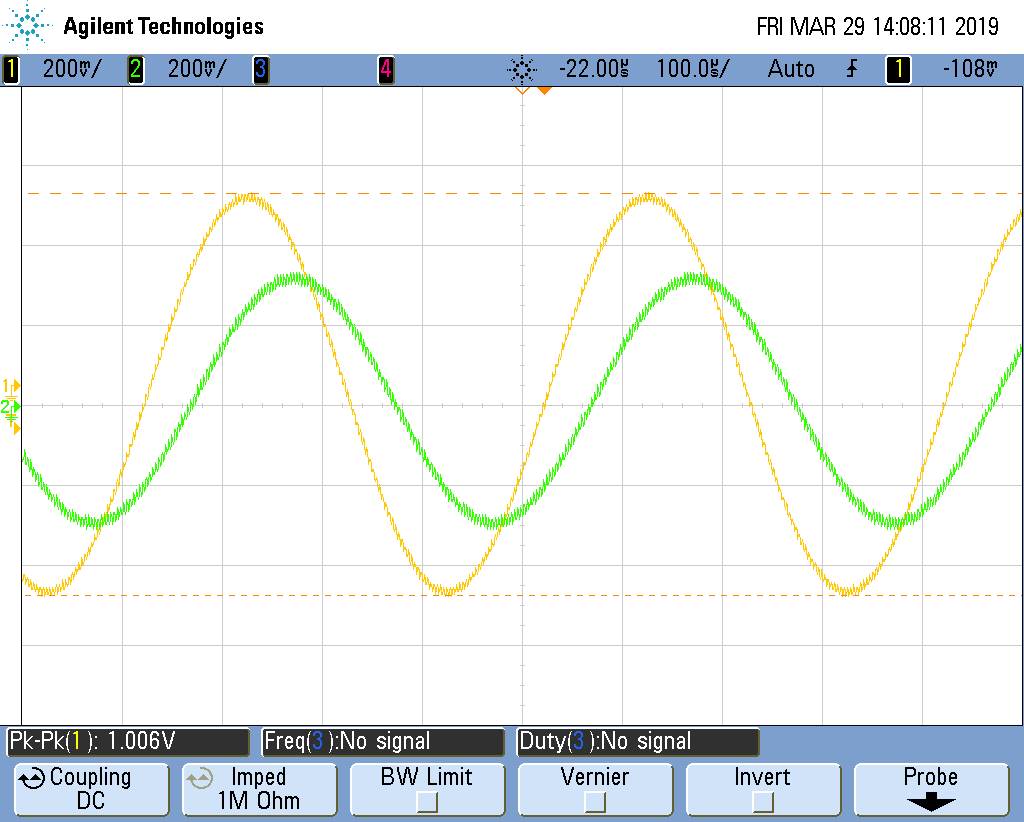
\includegraphics[scale=0.25]{Imagenes/llave_senooo_pto_a1}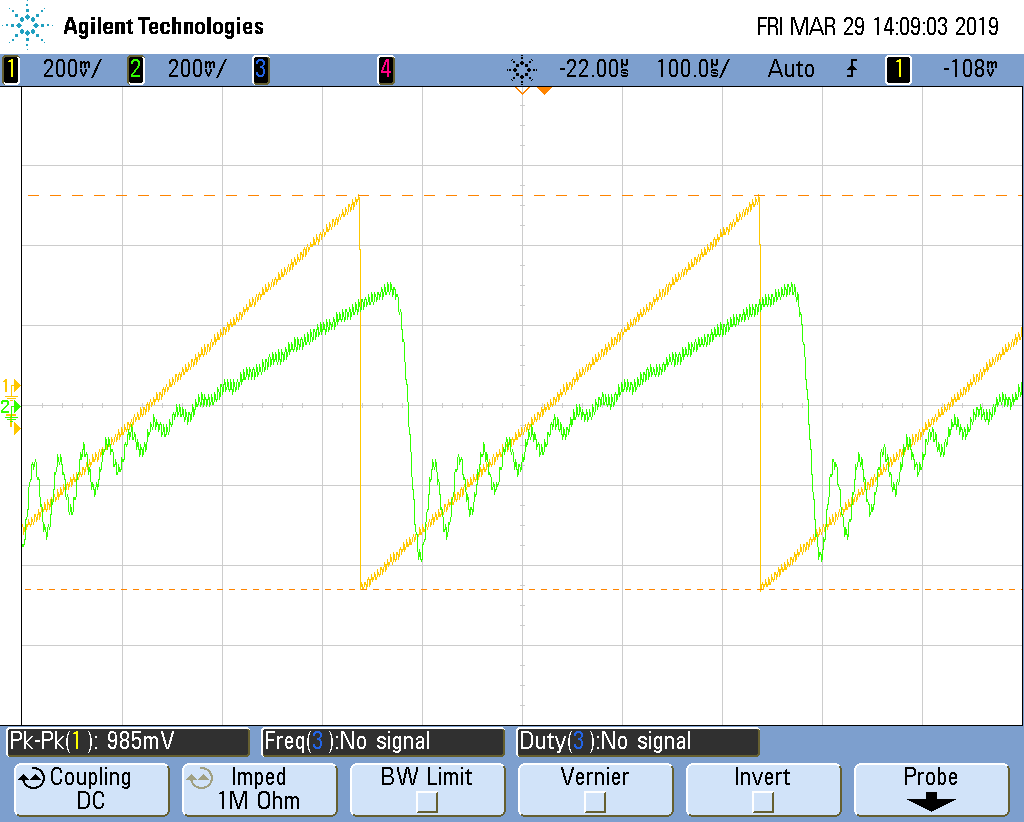
\includegraphics[scale=0.25]{Imagenes/llave_diente_pto_a}
\par\end{centering}
\centering{}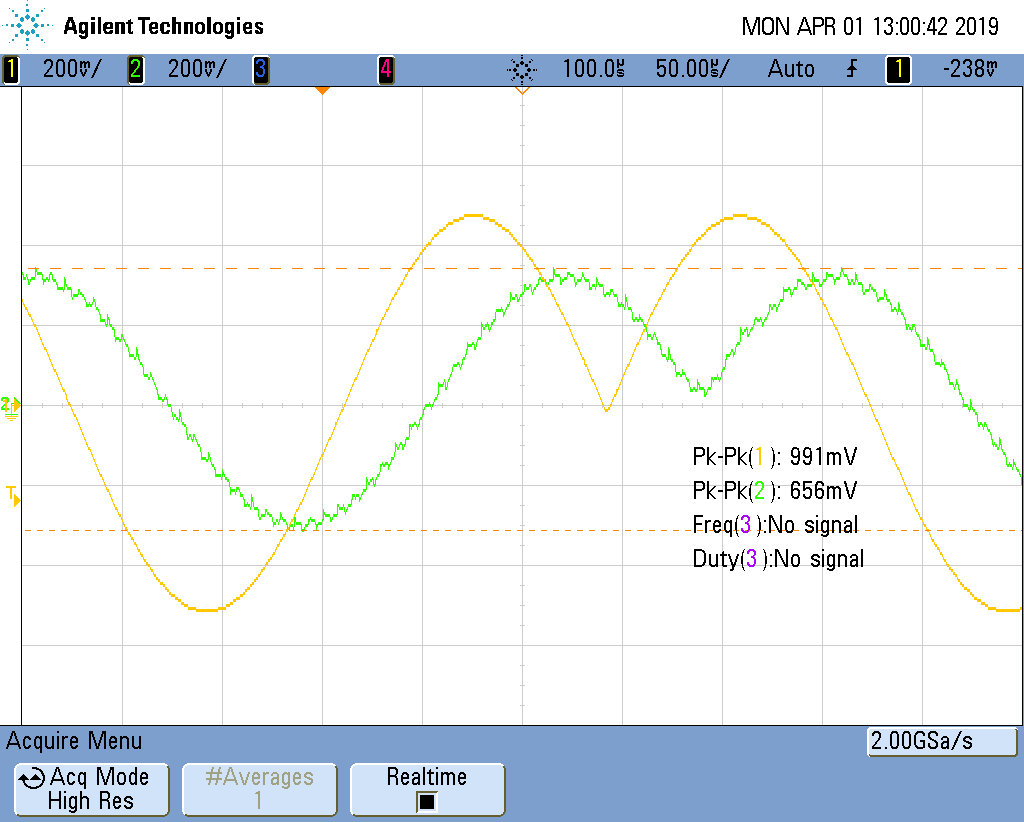
\includegraphics[scale=0.25]{Imagenes/ej_6_}\caption{De izq a der: salida (verde) de la placa con $X_{a}$; salida con
$X_{b}$; salida con $X_{c}$}
\end{figure}

Para la señal $X_{a}$, los valores óptimos que se obtuvieron fueron:
$f_{s}:[76,3;313](kHz)$midiendo en el máximo de ese intervalo, $DC=48.5\%,$$A:(0;2]$(Vpp)
midiendo para $A=1V_{pp}$.

Para la señal $X_{b}$, los valores óptimos obtenidos fueron: $f_{s}:[91;313](kHz)$midiendo
en el máximo de ese intervalo, $DC=48.8\%,$$A:(0;2]$(Vpp) midiendo
para $A=1V_{pp}$.

Para la señal $X_{c}$, los valores óptimos obtenidos fueron: $f_{s}:[80;300](kHz)$midiendo
en la frecuencia de 140kHz perteneciente a ese intervalo, $DC=49.8\%,$$A:(0;2]$(Vpp)
midiendo para $A=1V_{pp}$.

Para realizar un análisis más completo, hemos realizado una simulación
con igualdad de parámetros para poder contrastar las diferencias entre
los planos teóricos y prácticos. Podemos ver los resultados de dichas
simulaciones en la siguiente imagen:

\begin{figure}[H]

\begin{centering}
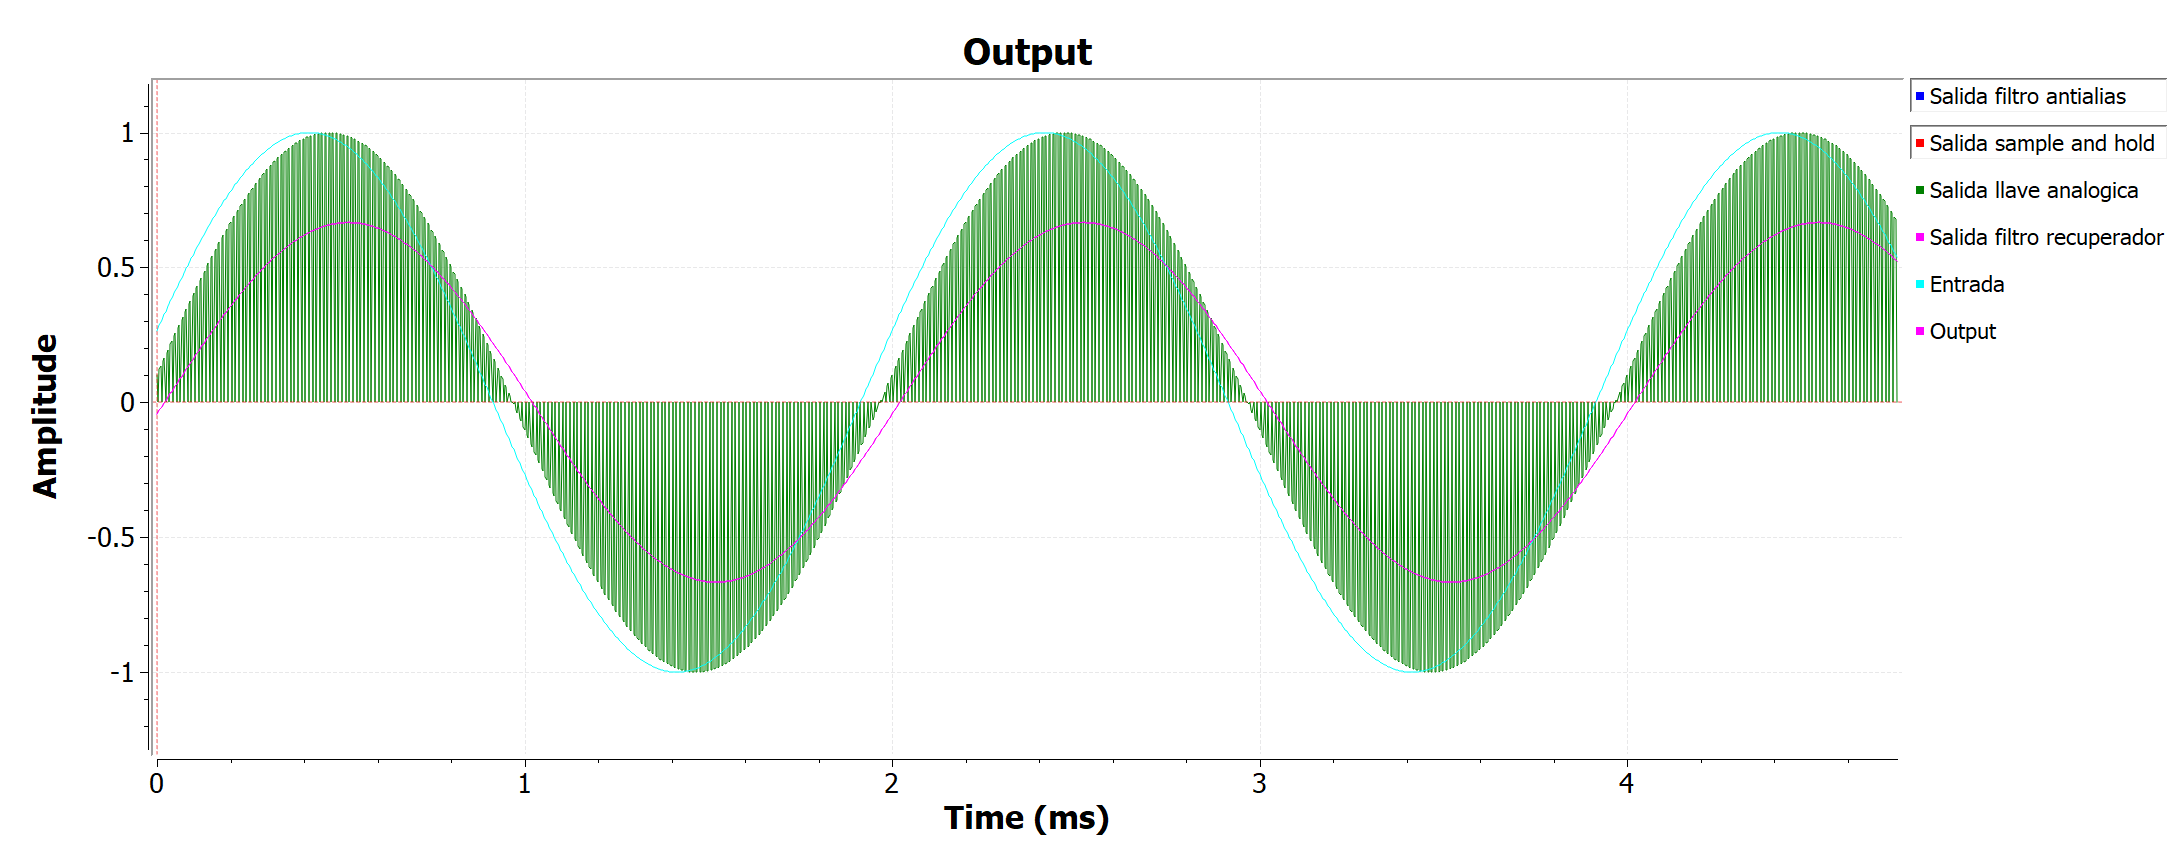
\includegraphics[scale=0.5]{Imagenes/simulacion_llave_seno_a.PNG}
\par\end{centering}
\begin{centering}
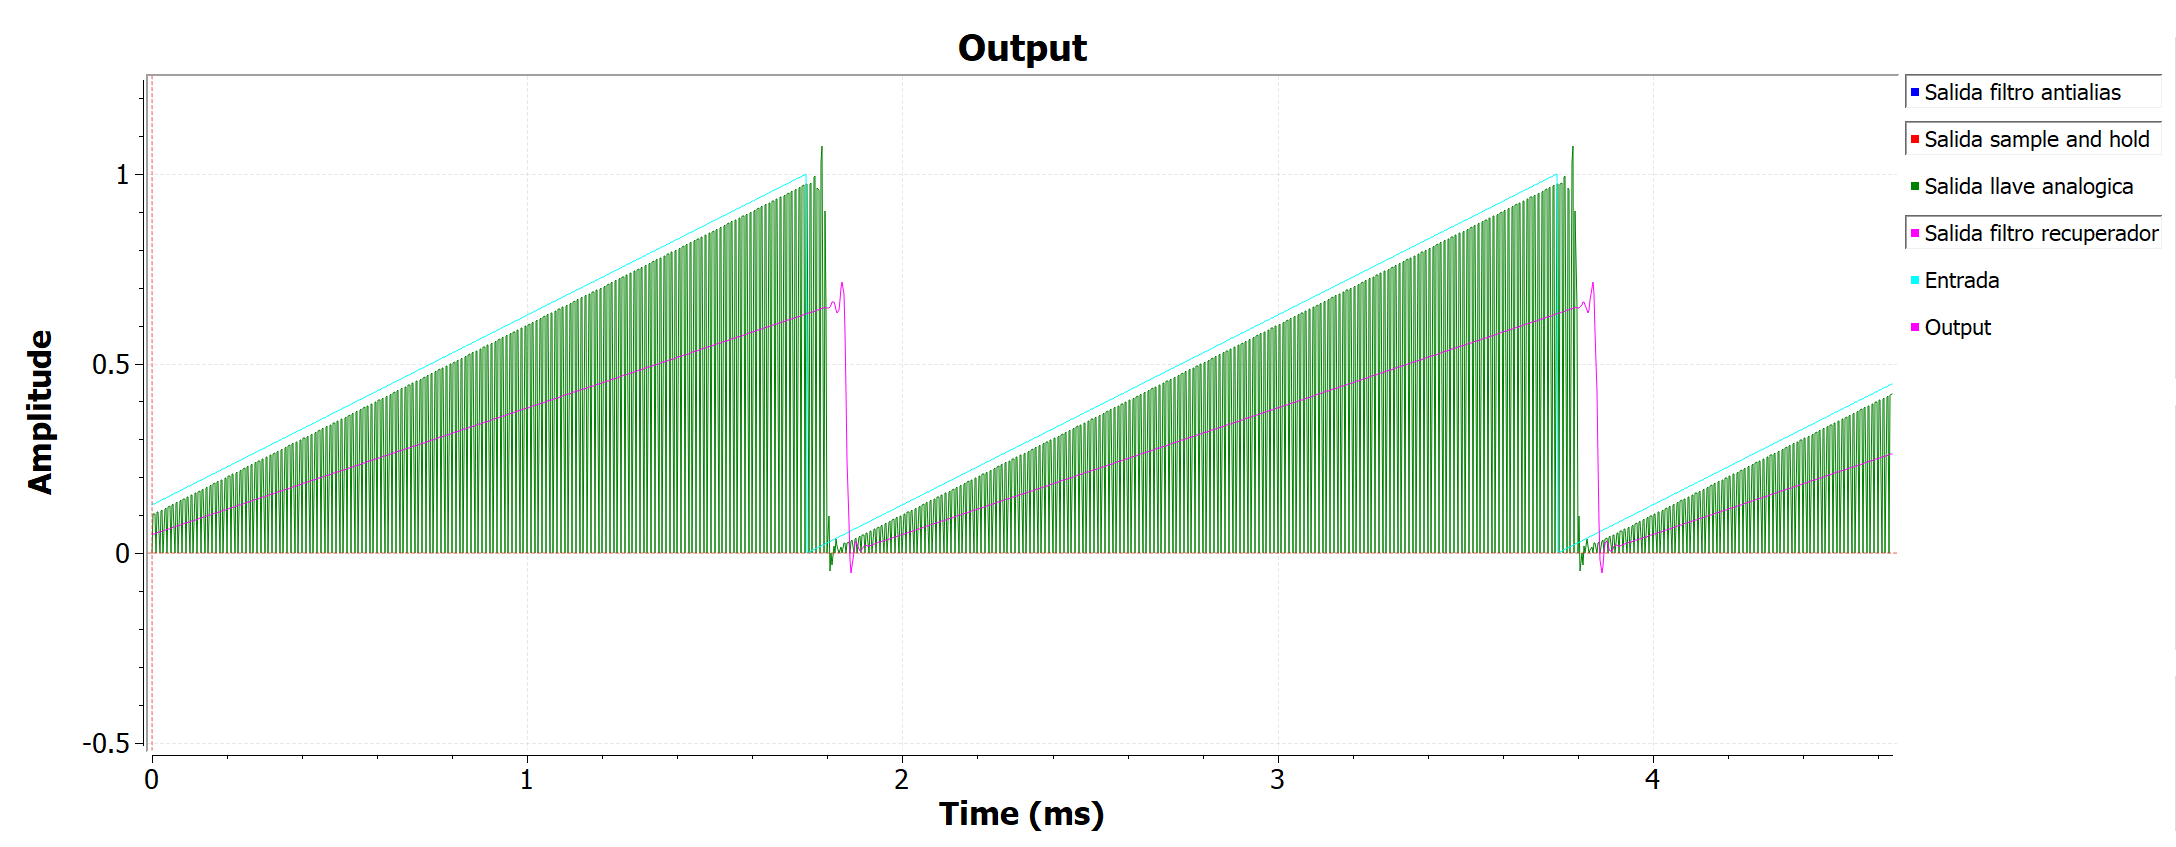
\includegraphics[scale=0.5]{Imagenes/simulacion_llave_diente_a.PNG}
\par\end{centering}
\begin{centering}
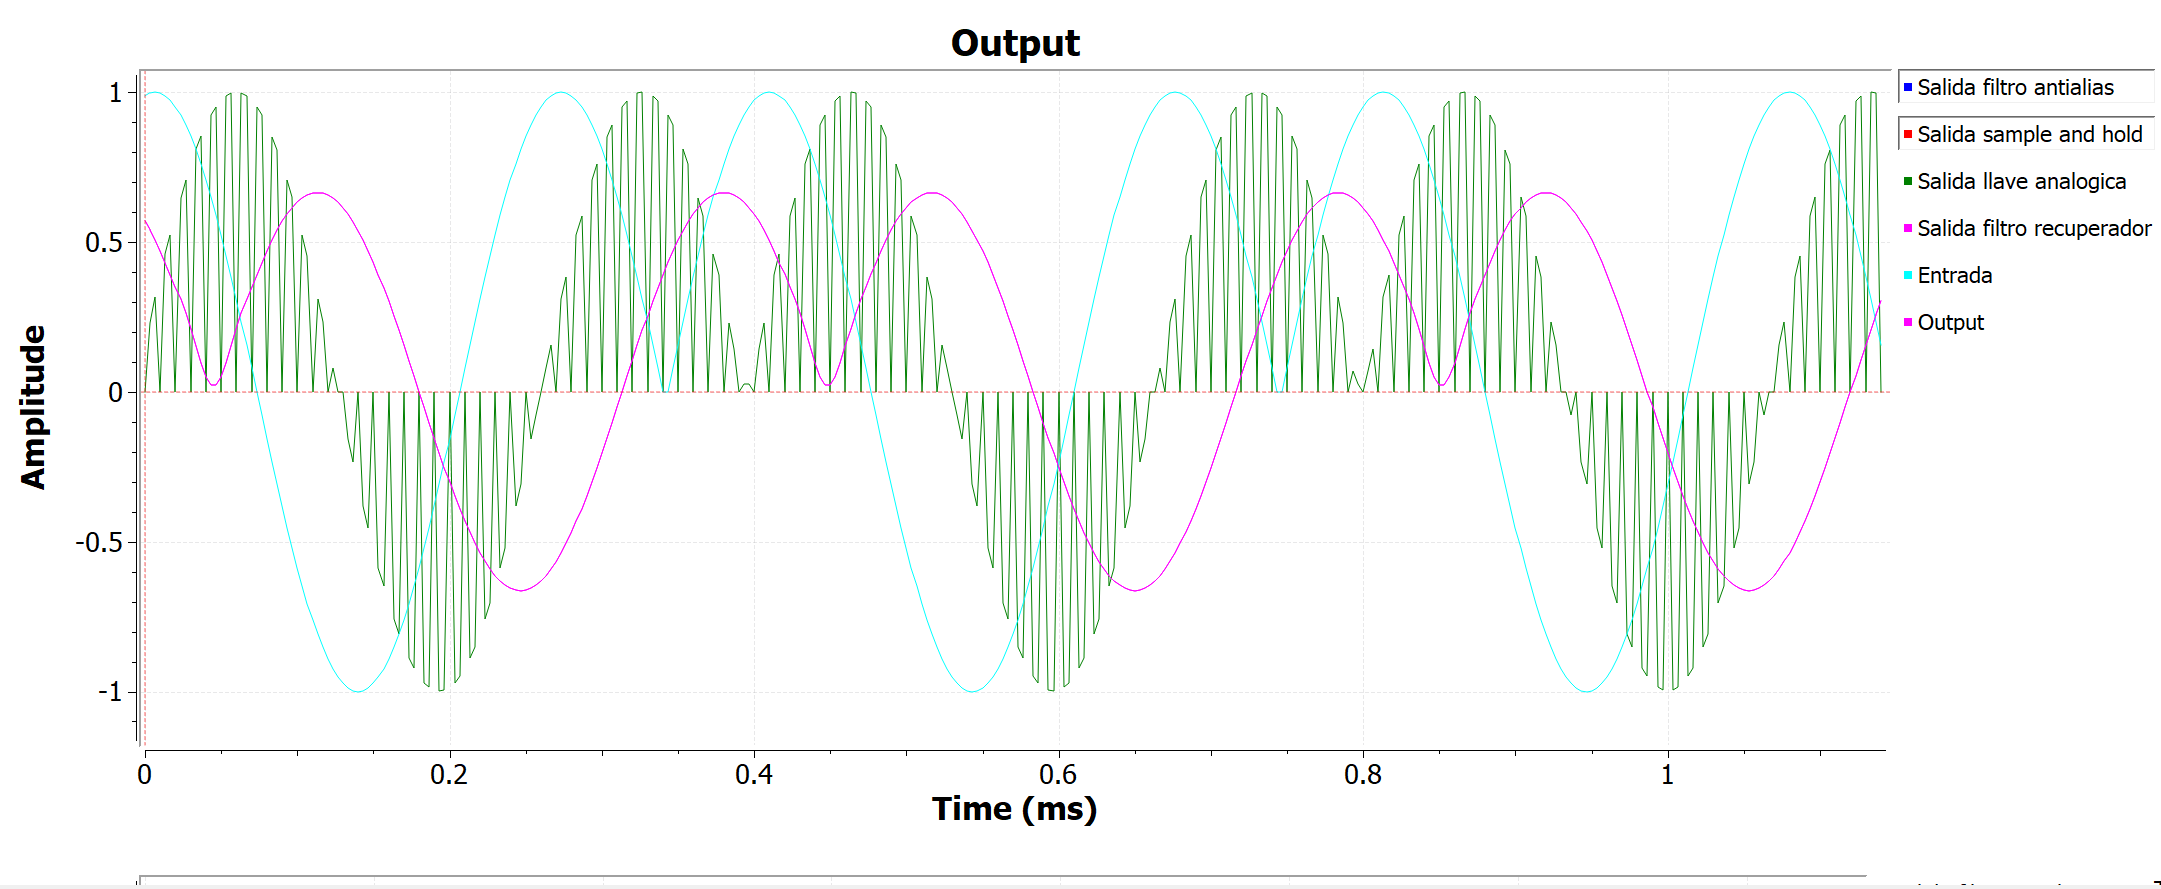
\includegraphics[scale=0.5]{Imagenes/simulacion_llave_senoraro_a.PNG}\caption{Simulaciones de las respuestas a las señales $X_{a}$ y $X_{b}$ }
\par\end{centering}
\end{figure}

A primera vista, podemos ver como se aprecian ciertas diferencias
entre el modelo teórico y el resultante en la práctica. Primero, observamos
como en el modelo teórico, la señal parece tener un ripple que el
osciloscopio no muestra, esto se debe a que en efecto en el modelo
teórico la recuperación de la señal está dada por funciones $\delta$,
mientras que en la placa se obtienen funciones sincs lo que hace que
aparezcan más valores.

\subsection{Cambios en la $f_{in}$ y en la $f_{s}$}

\subsubsection{$f_{in}<\frac{f_{p}}{2}$,$f_{s}=f_{a}$}

Para este caso, se exitó a la placa con una señal $X_{a}$, con la
diferencia respecto al punto anterior de que ahora el rango de $f_{in}=(0;45]$(kHz)
y la $f_{s}=68kHz.$Con el nuevo intervalo de $f_{in}$, finalmente
se eligió $f_{in}=500Hz.$ El duty cycle utilizado fue de 47.6\%.

Para la señal $X_{b}$, por otra parte el rango de $f_{in}$ pasó
a ser $f_{in}=(0;45]$(kHz) y la $f_{s}$ mantuvo su valor de $68kHz.$Con
el nuevo intervalo de $f_{in}$, finalmente se eligió $f_{in}=500Hz.$
El duty cycle utilizado también fue de 47.6\%.

Para la señal $X_{c},$el rango de $f_{in}$ disminuyó hasta los valores
$f_{in}=(0;3.9]$(kHz) con un DC de 49.8\%. Se midió a una frecuencia
de 500Hz.

Los resultados se ven plasmados en la siguiente image:

\begin{figure}[H]

\begin{centering}
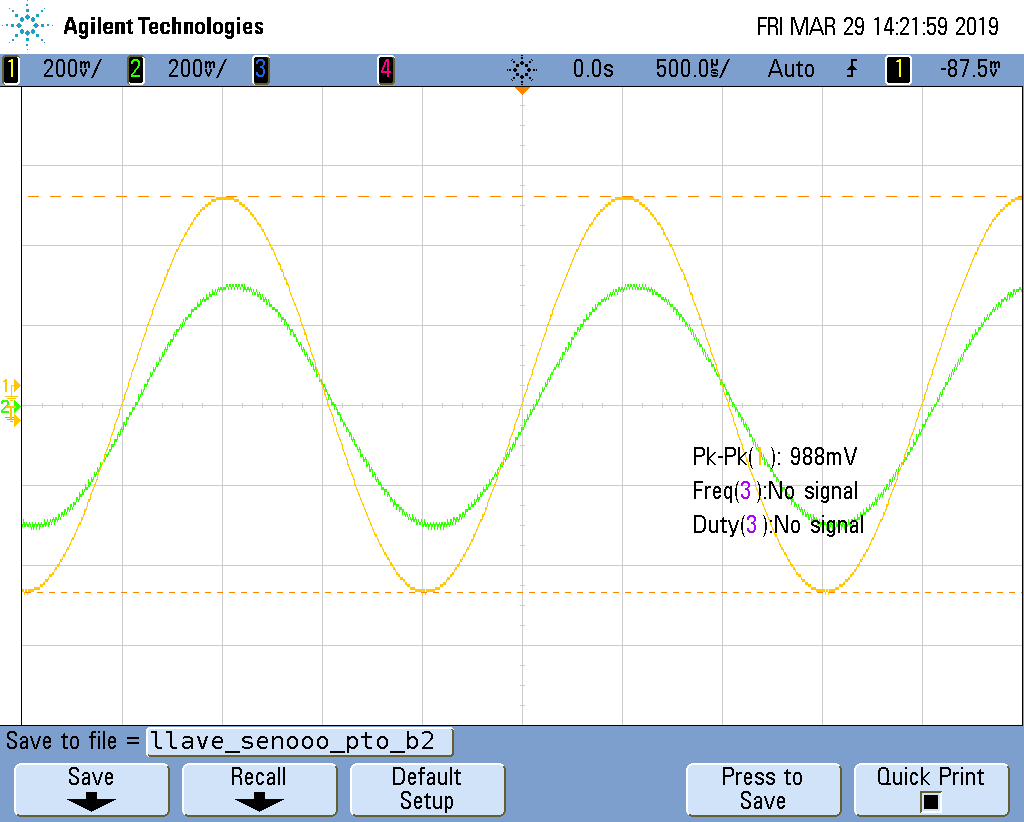
\includegraphics[scale=0.25]{Imagenes/llave_senooo_pto_b2}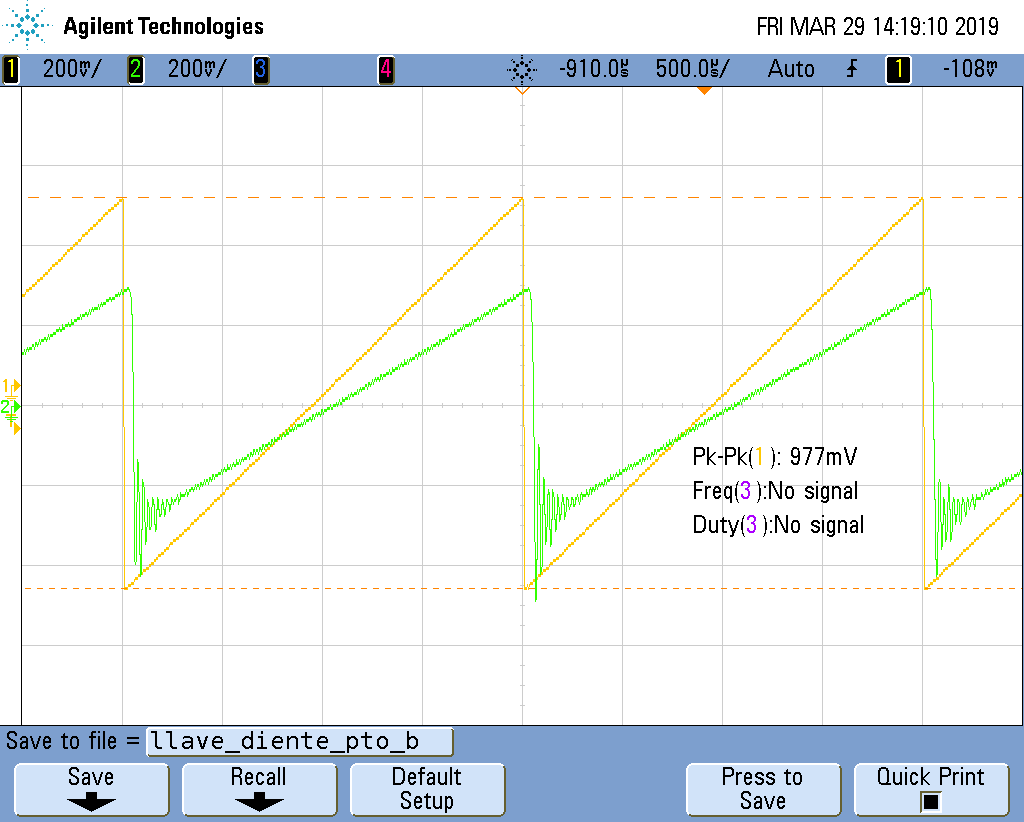
\includegraphics[scale=0.25]{Imagenes/llave_diente_pto_b}
\par\end{centering}
\centering{}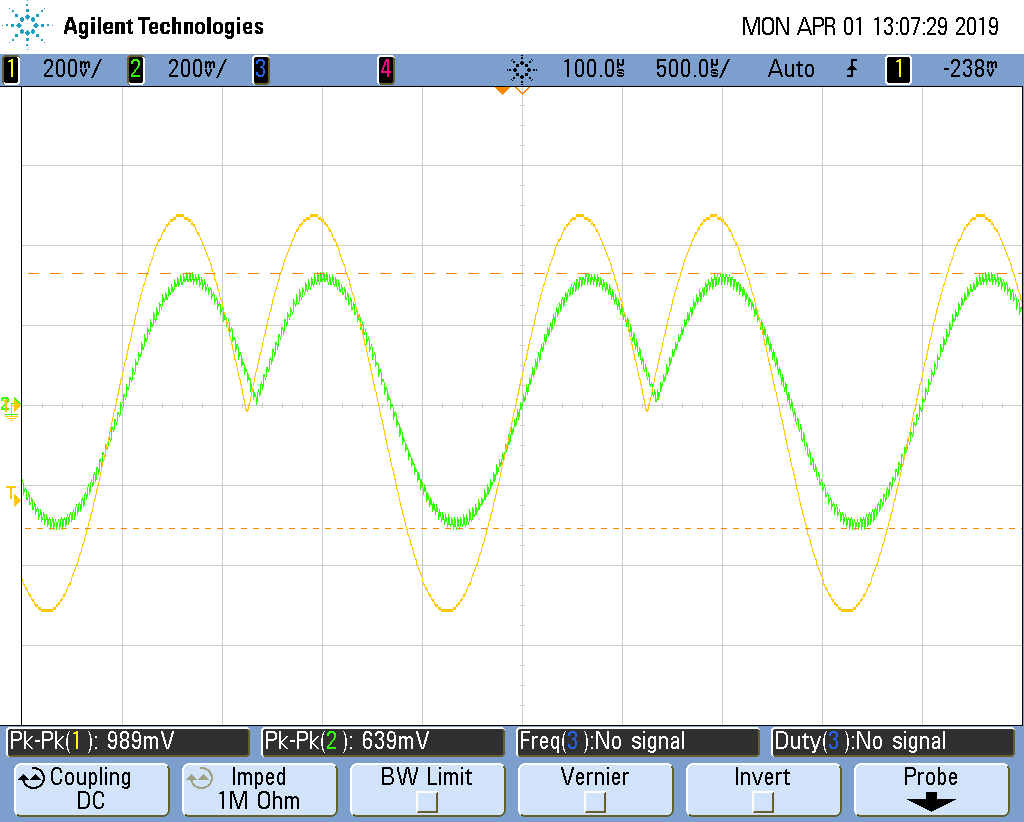
\includegraphics[scale=0.25]{Imagenes/ej_6_b_}\caption{De izquierda a derecha: señal $X_{a}$; señal $X_{b}$; y señal $X_{c}$.}
\end{figure}

Si contrastamos con las simulaciones pertinentes, las cuales se muestran
a continuación, no se observan diferencias significativas, más alla
de la intensificación del ripple en la salida, y de la atenuación
pertinente que sufre cada señal.

\begin{figure}[H]

\begin{centering}
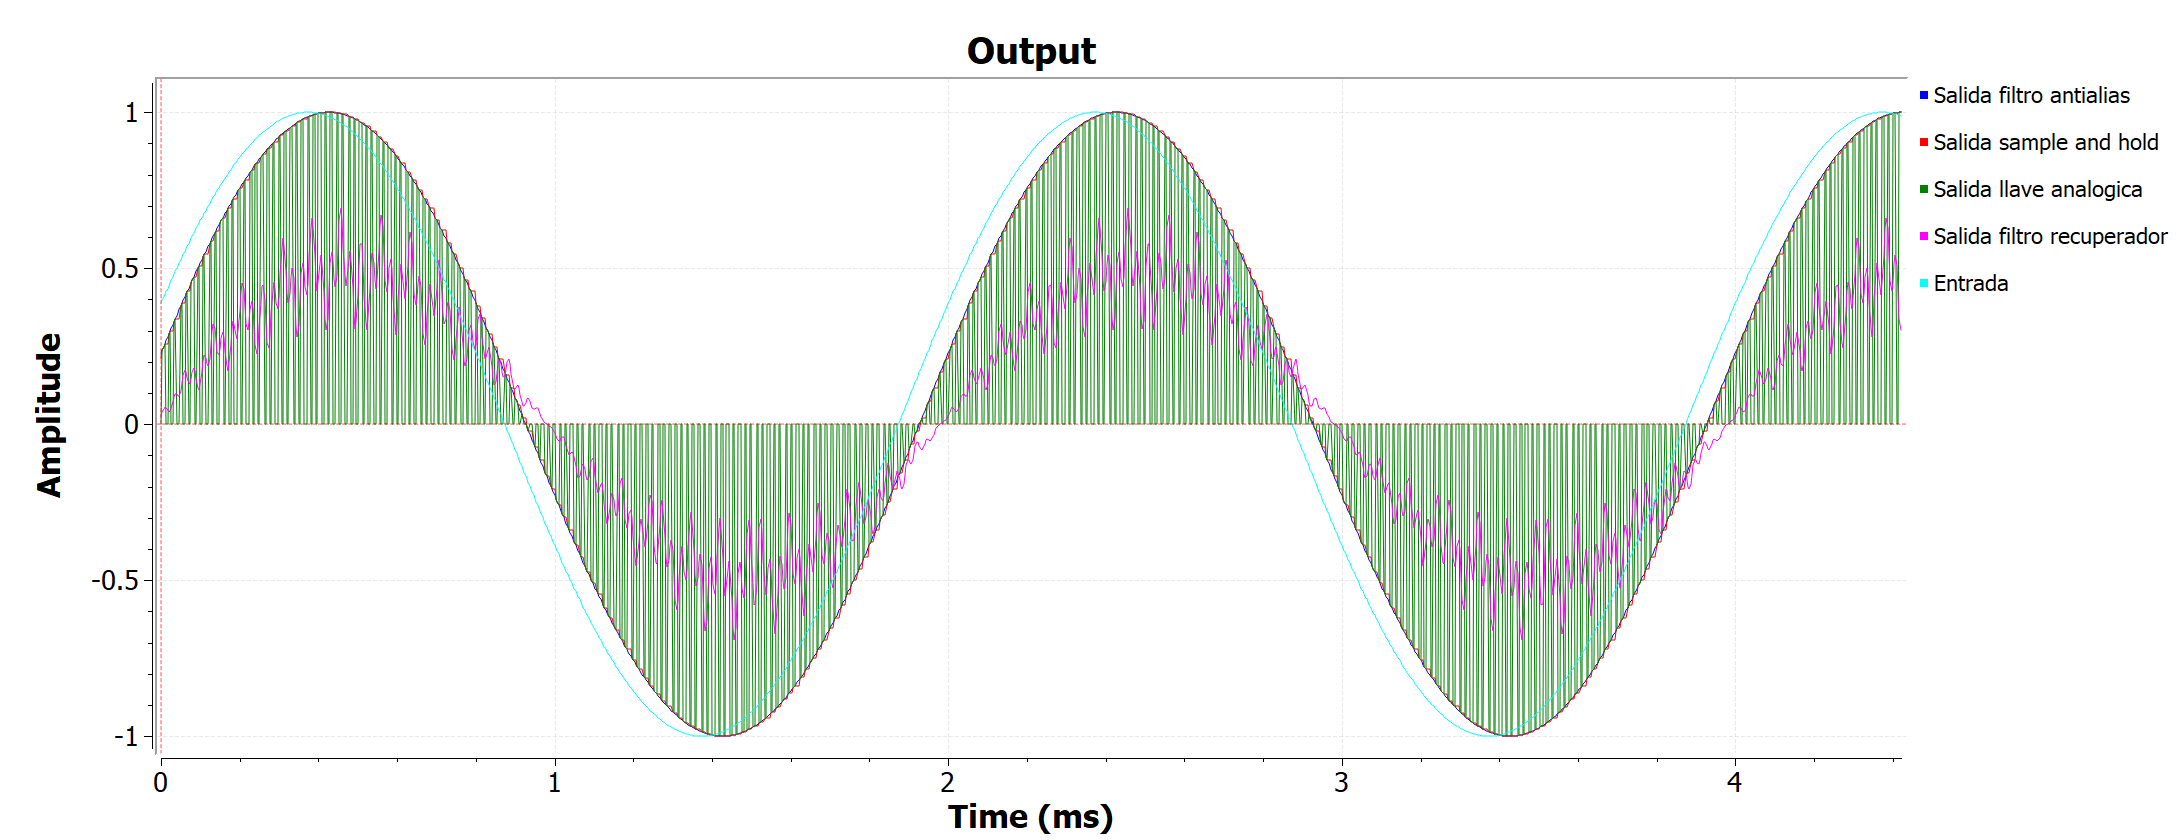
\includegraphics[scale=0.5]{Imagenes/simulacion_llave_seno_b1.PNG}
\par\end{centering}
\begin{centering}
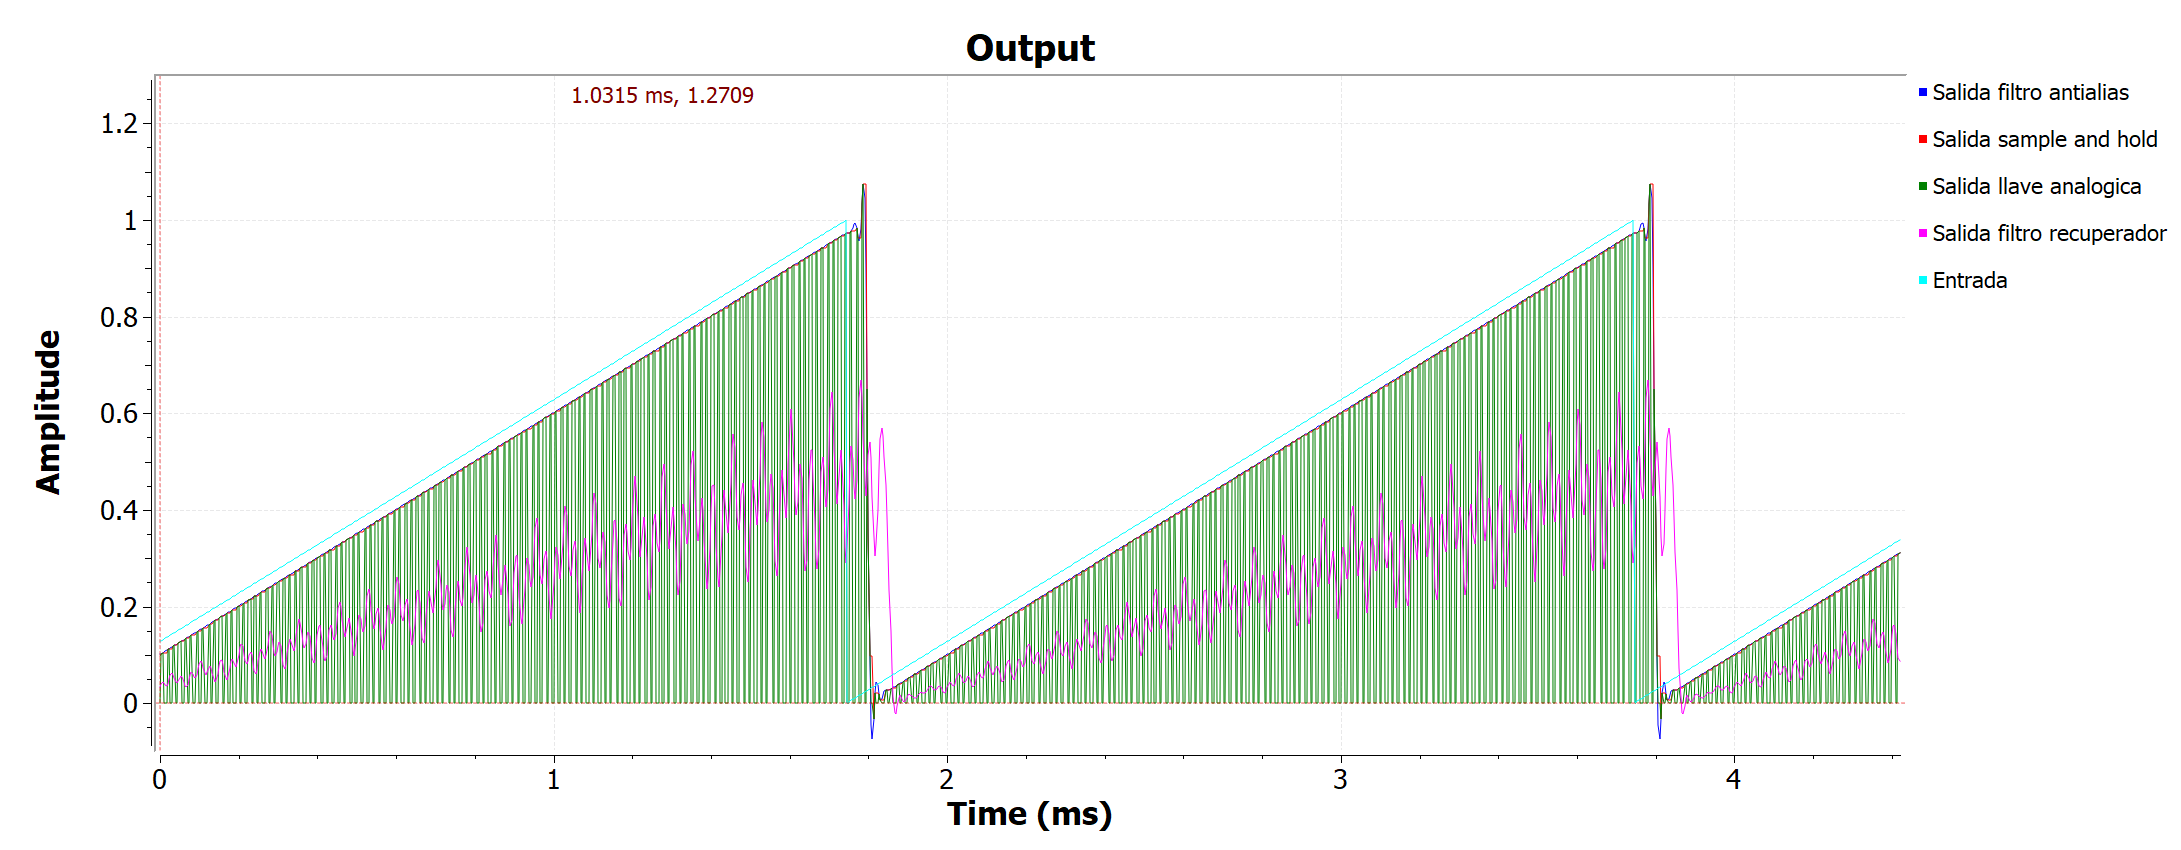
\includegraphics[scale=0.5]{Imagenes/simulacion_llave_diente_b1.PNG}
\par\end{centering}
\begin{centering}
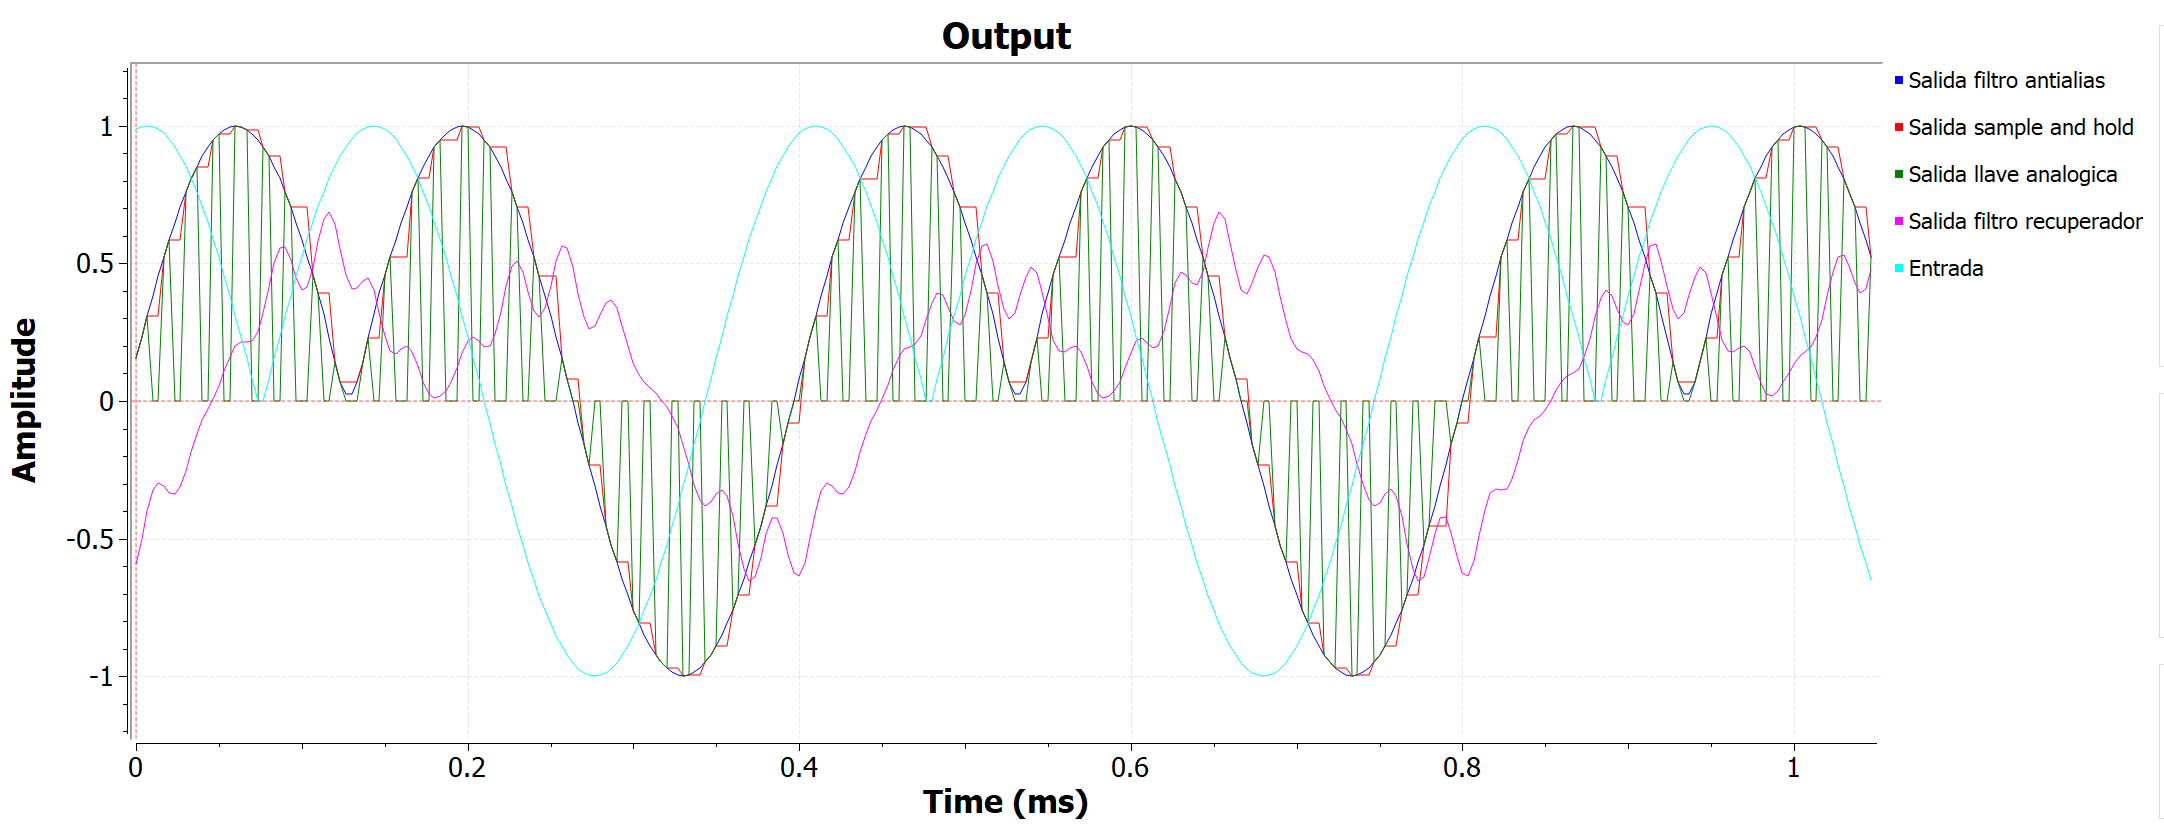
\includegraphics[scale=0.5]{Imagenes/simulacion_llave_senoraro_b1.PNG}\caption{Simulaciones de la señal $X_{a}$y señal $X_{b}$ }
\par\end{centering}
\end{figure}


\subsubsection{$f_{in}=f_{a}$}

Para este punto, tanto a la señal $X_{a}$ como $X_{b}$ y $X_{c}$,
se las estableció con una frecuencia $f_{in}=68kHz$. Para la frecuencia
de muestreo, se optó por utilizar la máxima posible, es decir $f_{s}=313kHz.$Para
ambas señales, se mantuvo el mismo duty cycle de 48\%. Los resultados
pueden ser apreciados en la siguiente imagen:

\begin{figure}[H]

\begin{centering}
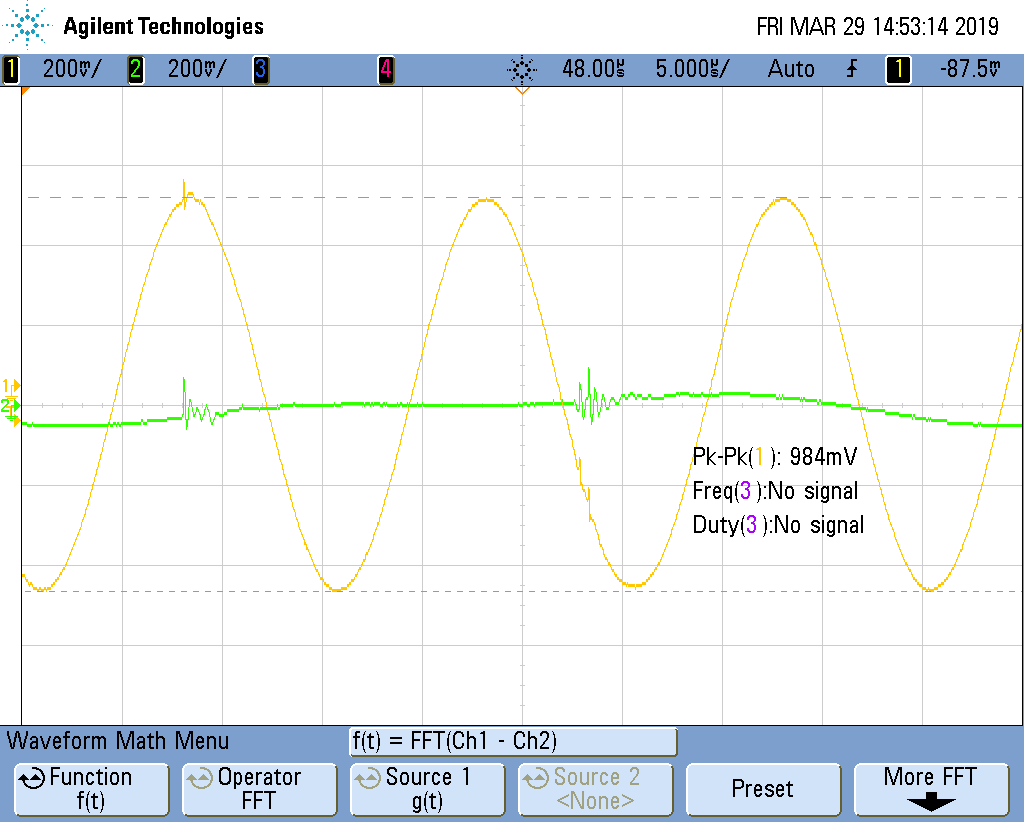
\includegraphics[scale=0.25]{Imagenes/llave_senooo_pto_bf1}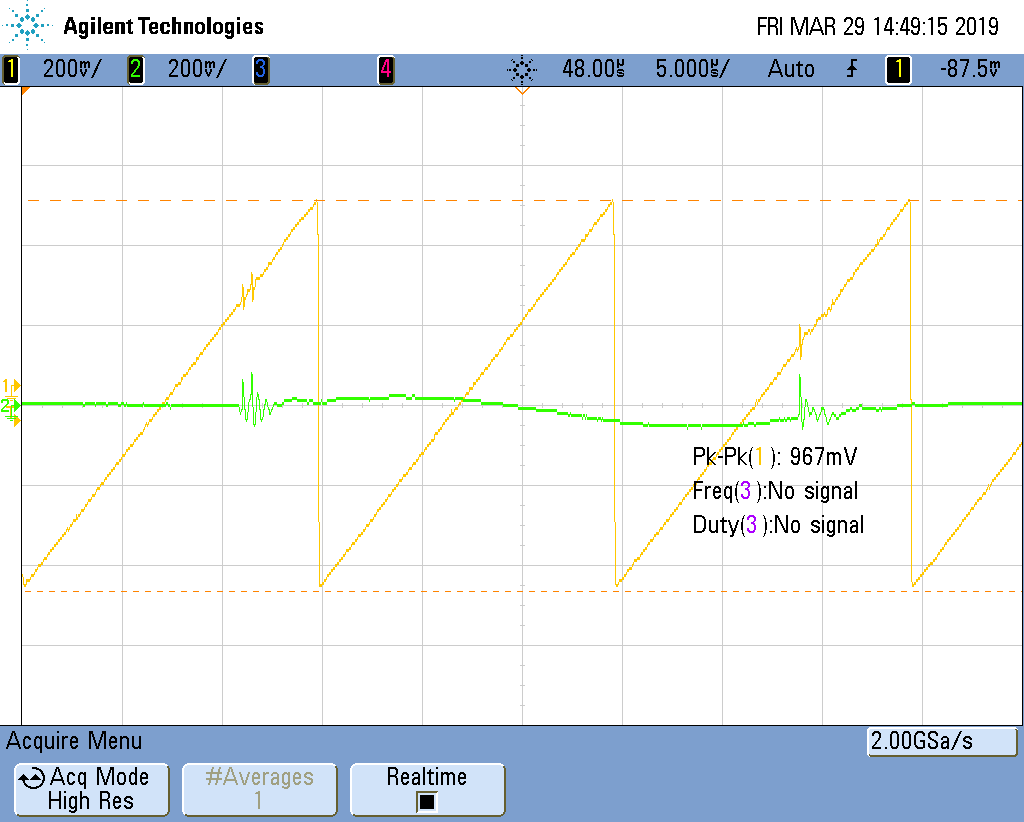
\includegraphics[scale=0.25]{Imagenes/llave_djente_pto_bfa}
\par\end{centering}
\begin{centering}
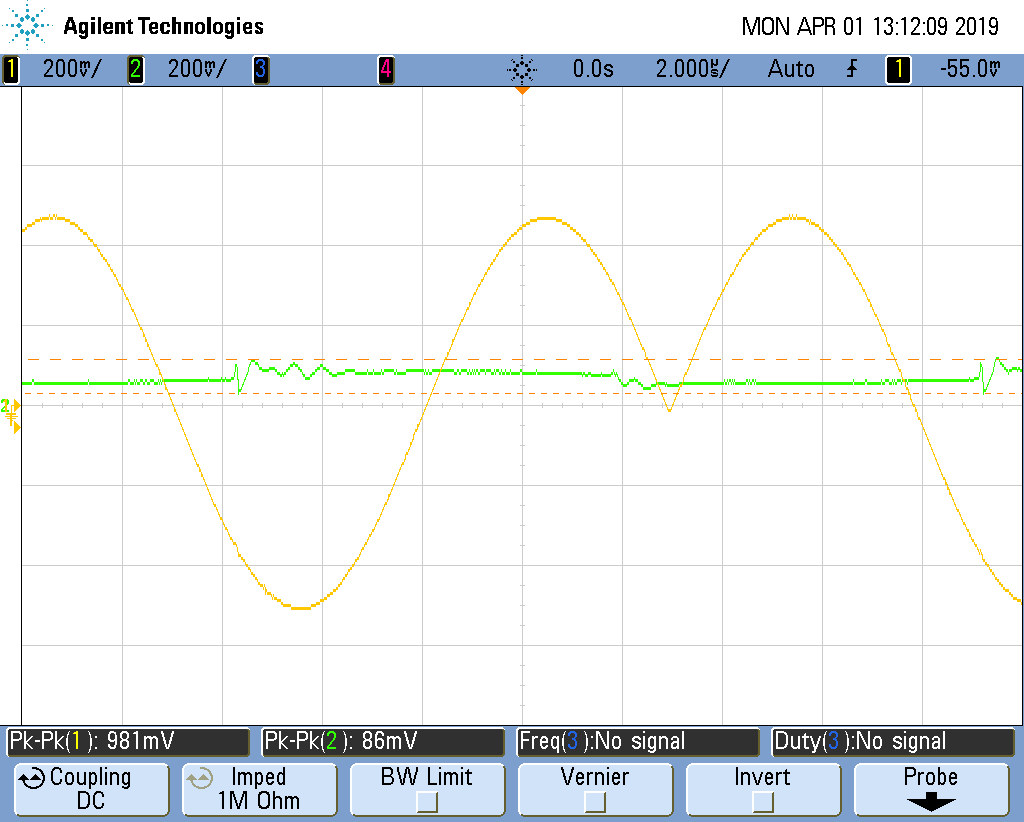
\includegraphics[scale=0.25]{Imagenes/ej_6_b_2}\caption{De izquierda a derecha: señal $X_{a}$; señal $X_{b}$ y señal $X_{c}$.}
\par\end{centering}
\end{figure}

Resultados similares nos arroja la simulación realizada, en la cual
si bien las gráficas de la simulación se ven ``estéticamente'' afectadas
por el hecho de la cantidad de puntos que se incorporaron en la imagen,
lo cierto es que en ambos casos la señal saliente resulta nula para
el caso de la senoidal, e igualmente para el caso de la función rampa
con la salvedad de que en vista de que el contenido armónico es mayor,
no es exactamente cero lo que se aprecia, sino que se tiene algo de
ruido a la salida.

\begin{figure}[H]

\begin{centering}
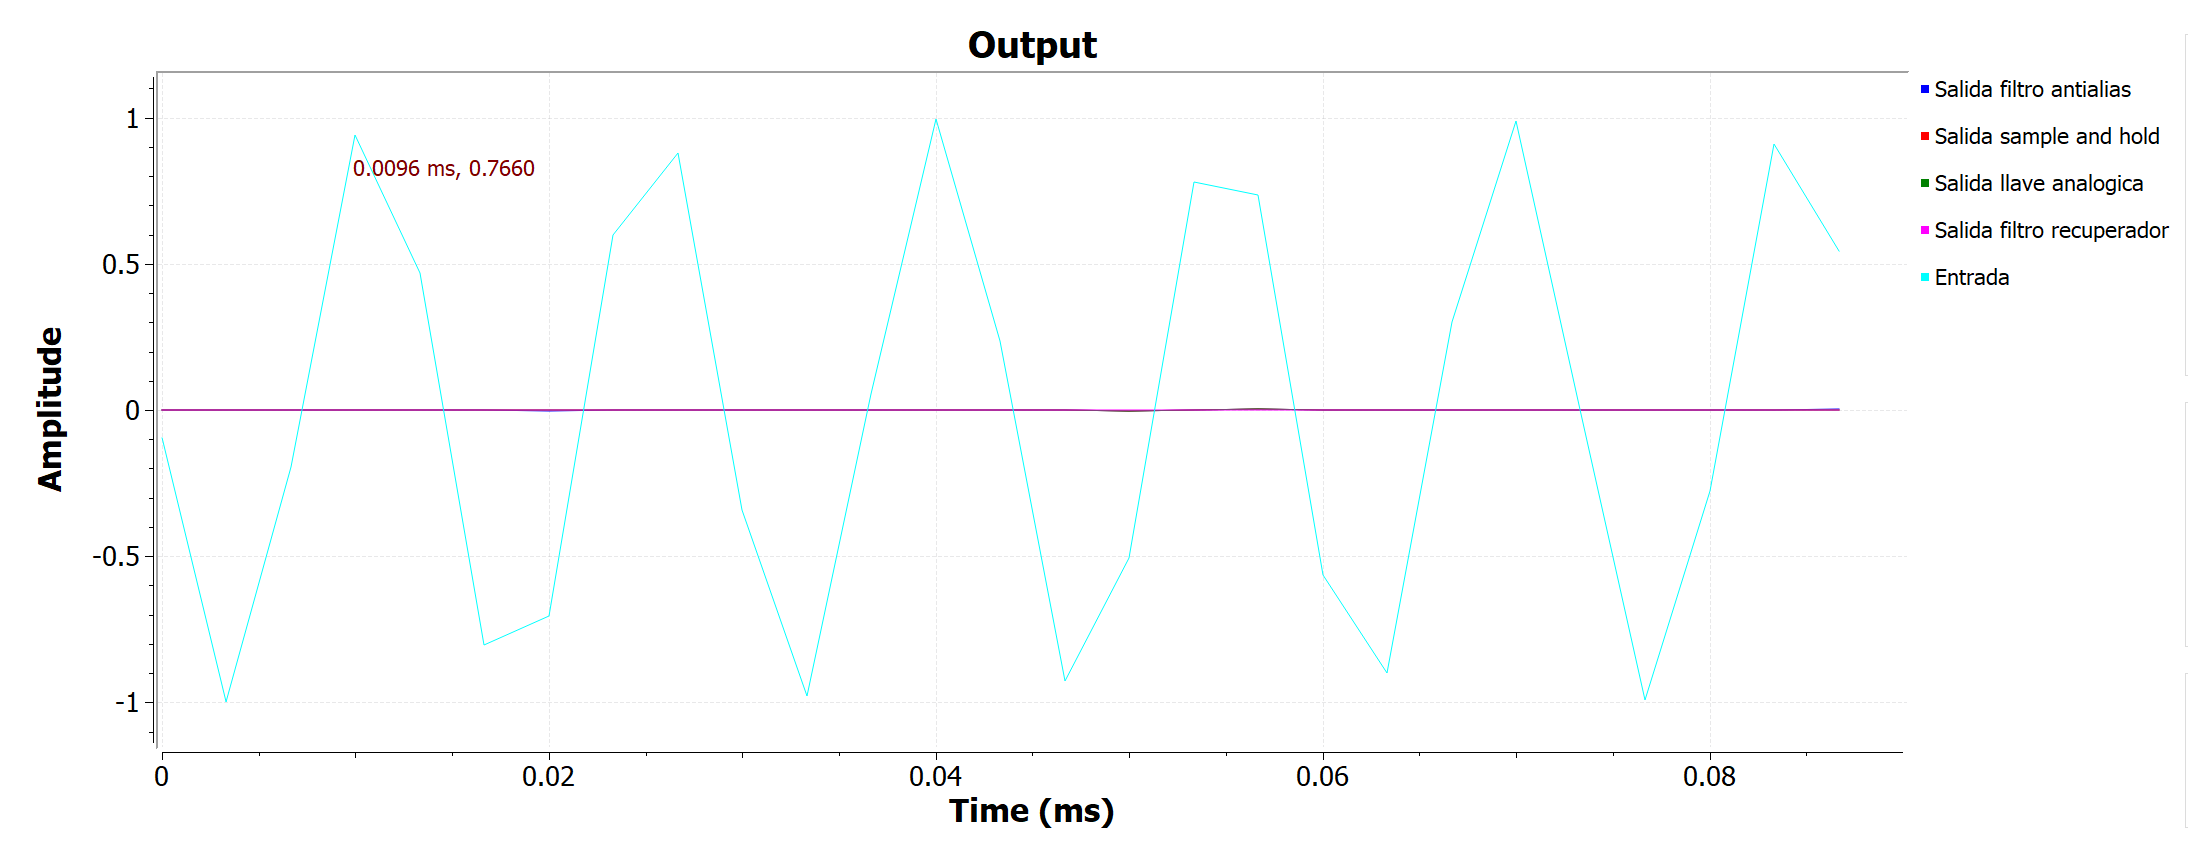
\includegraphics[scale=0.5]{Imagenes/simulacion_llave_seno_b2.PNG}
\par\end{centering}
\begin{centering}
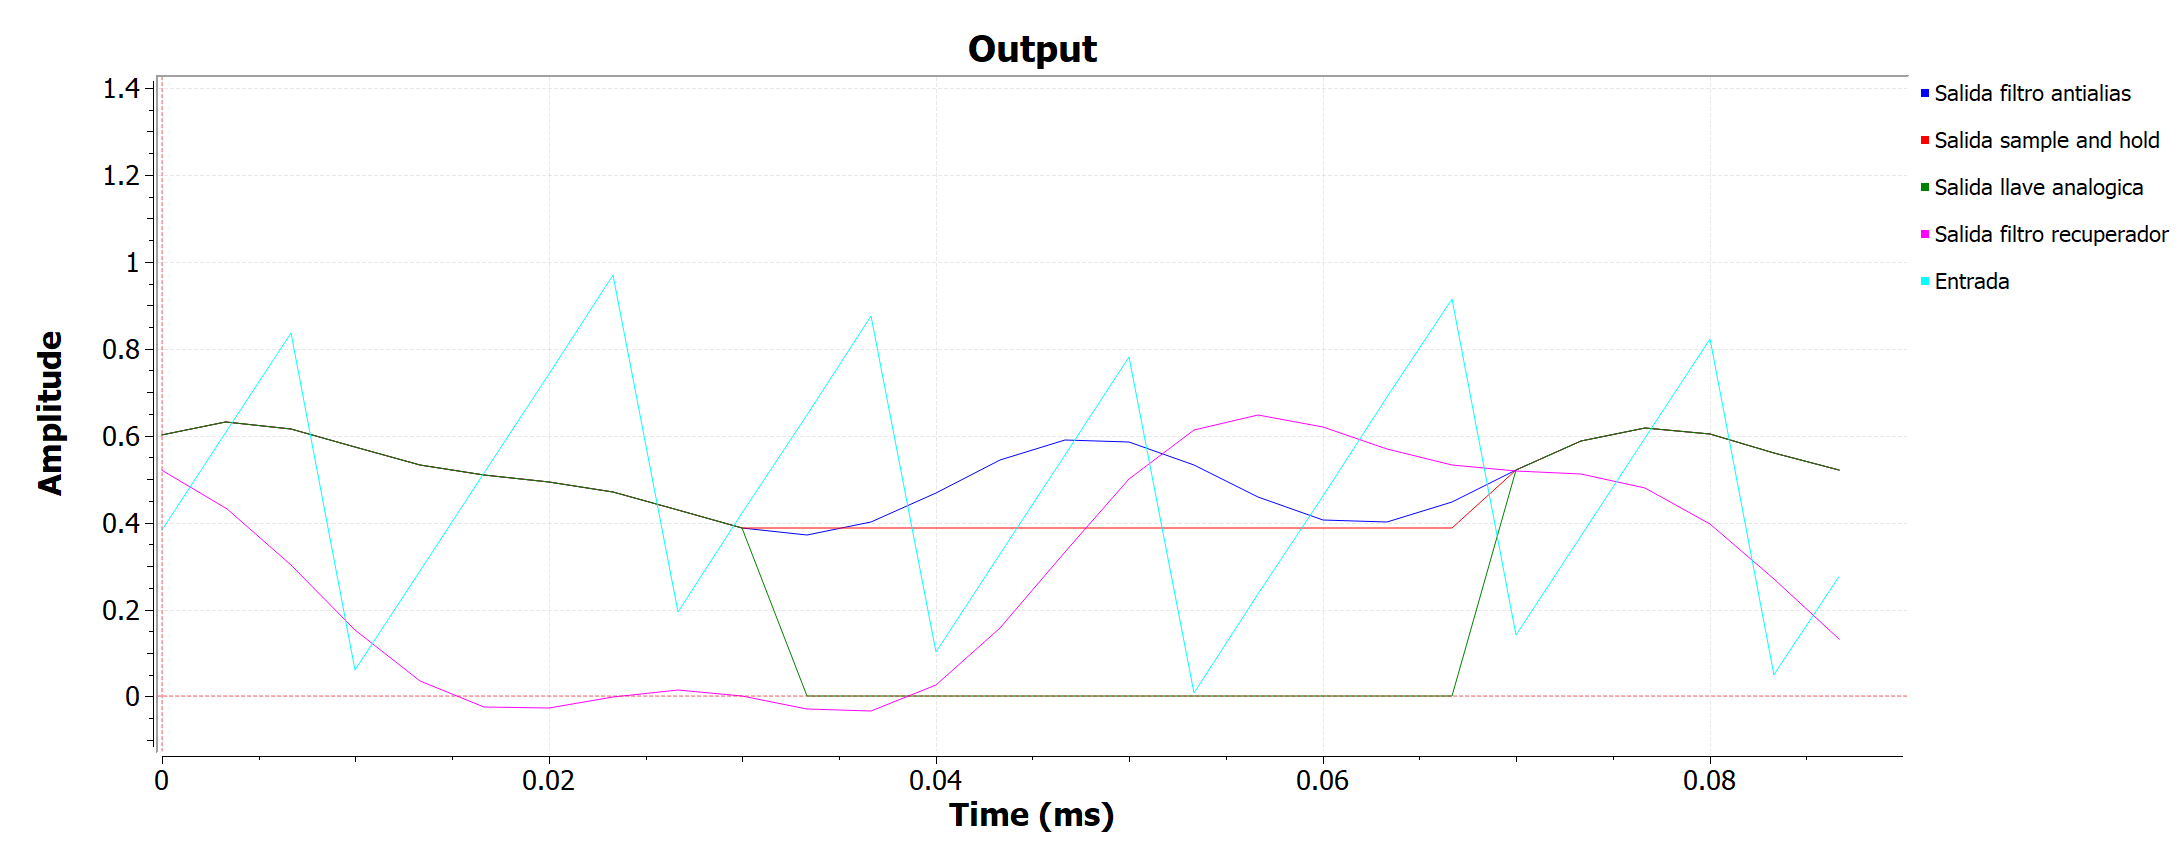
\includegraphics[scale=0.5]{Imagenes/simulacion_llave_diente_b2.PNG}
\par\end{centering}
\centering{}\caption{Simulaciones de la señal $X_{a}$y señal $X_{b}$ en iguales condiciones.}
\end{figure}


\subsection{$f_{in}=f_{s}\protect\leq f_{p}$}

Para este caso, solamente se exito al circuito con la señal $X_{a}$
con la particularidad que la frecuencia de la señal coincide con la
frecuencia de sampleo. Para ello, se optó por utilizar $f_{in}=f_{s}=10kHz$
y un DC de 47.3\%. La salida resultante se aprecia a continuación:

\begin{figure}[H]
\begin{centering}
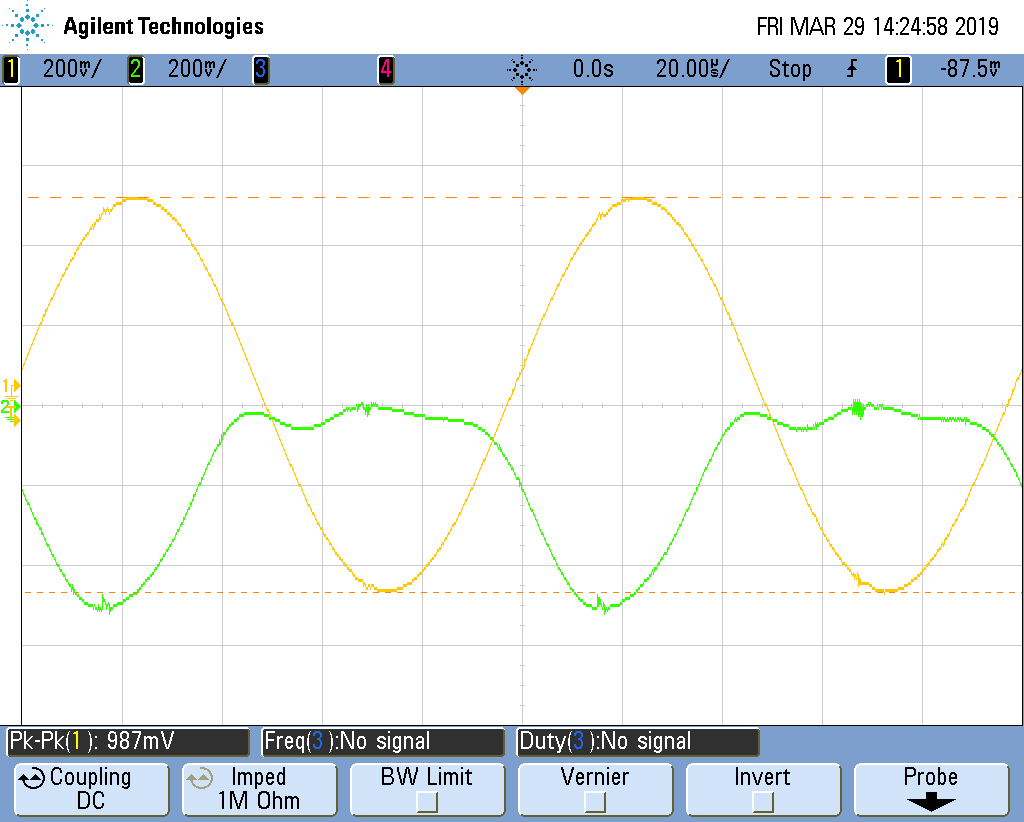
\includegraphics[scale=0.3]{Imagenes/llave_senooo_pto_c}\caption{Señal $X_{b}$ con frecuencia de muestreo igual a la de la señal.}
\par\end{centering}
\end{figure}

\begin{figure}[H]

\begin{centering}
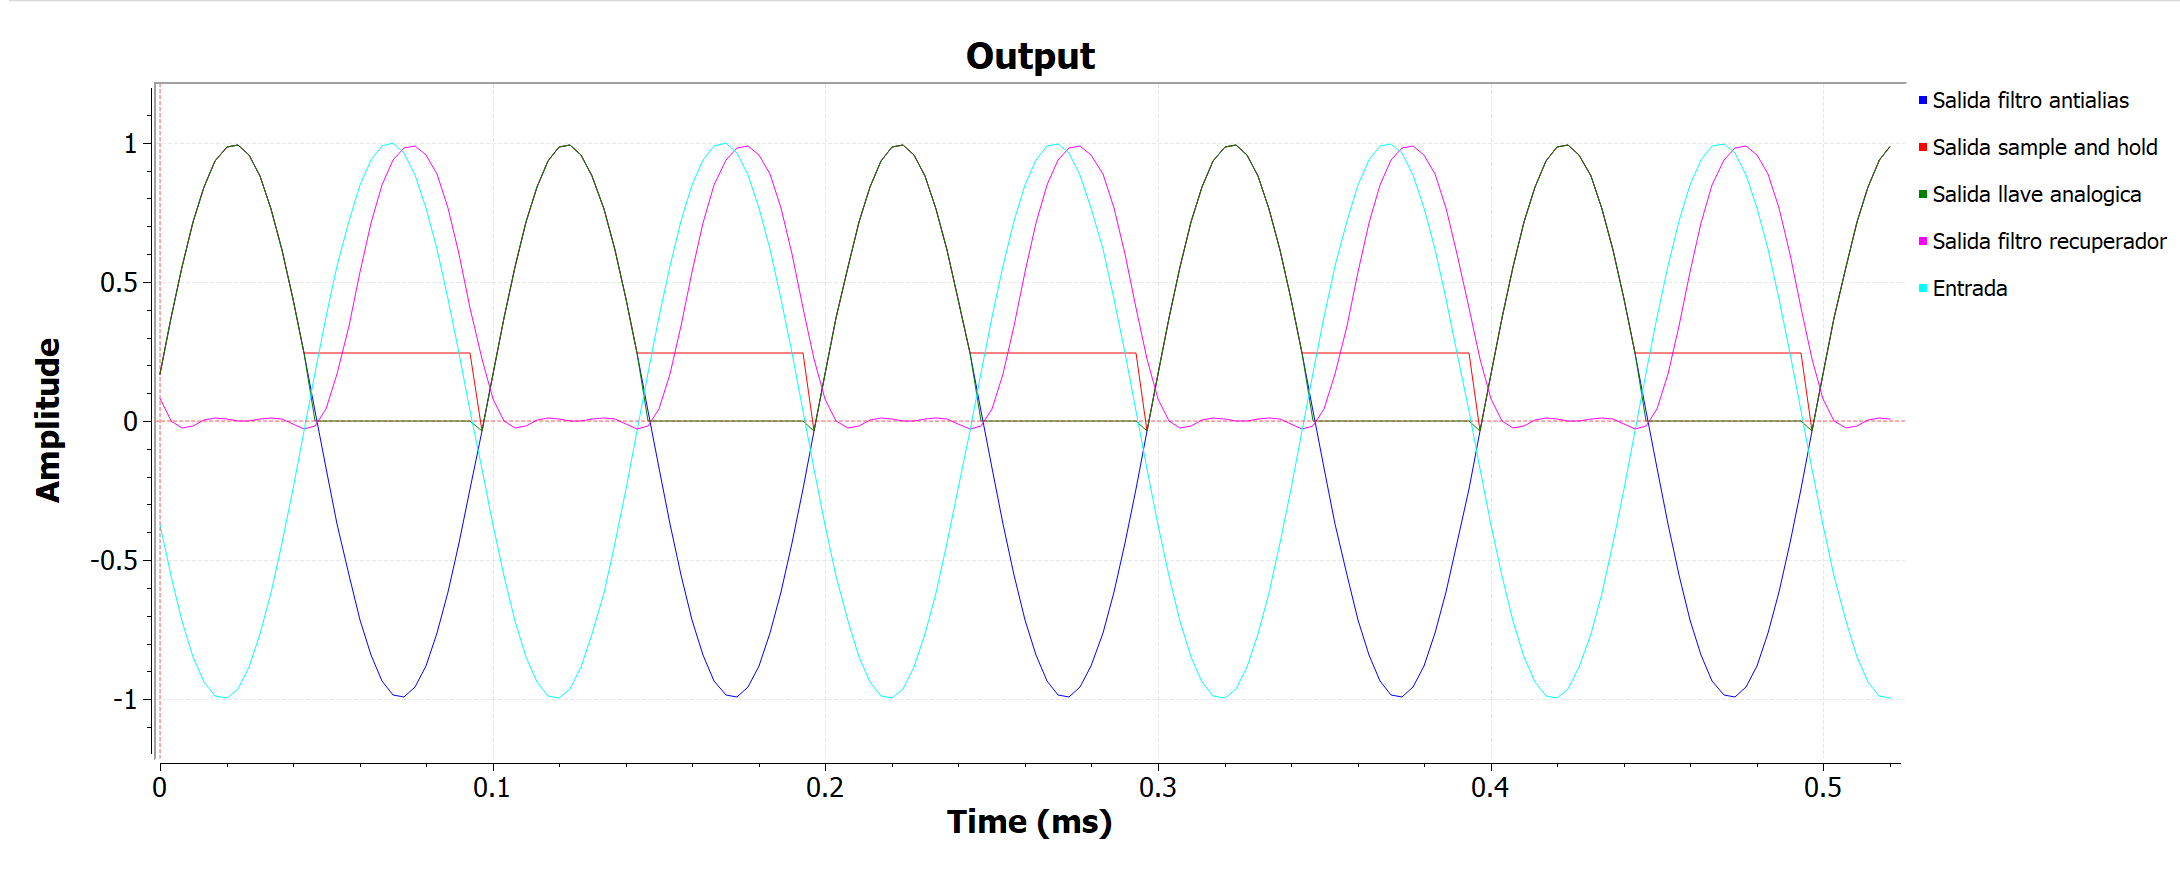
\includegraphics[scale=0.5]{Imagenes/simulacion_llave_seno_c.PNG}\caption{Simulación de la señal $X_{b}$.}
\par\end{centering}
\end{figure}

A la hora de contrastar con la simulación, notamos que se obtiene
la misma forma de la señal en ambos casos, solo que en la simulación
la señal queda definida positivamente, a diferencia de lo que ocurre
en el osciloscopio. Esto se debe a que la simulación no contempla
el desfasaje que el filtro le inyecta a las distintas frecuencias.

\subsection{Aliasing}

Para esta úlitma medición con la llave analógica, se exitó al circuito
con las señales $X_{b}$ y $X_{c}$variando sus frecuencias $f_{in}$
de manera tal de poder encontrar a qué frecuencia comienzan a aparecer
problemas de aliasing. Configurando las señales a una $f_{in}=2.5kHz,$observamos
que el efecto de aliasing aparece para la primera señal cuando la
frecuencia de esta cumple que $f_{s}<45kHz$.Para la señal $X_{c}$
se produce aliasing cuando $f_{s}<41.7kHz$ con un DC de 41.7\%. Podemos
ver los efectos en la siguiente imagen:

\begin{figure}[H]
\begin{centering}
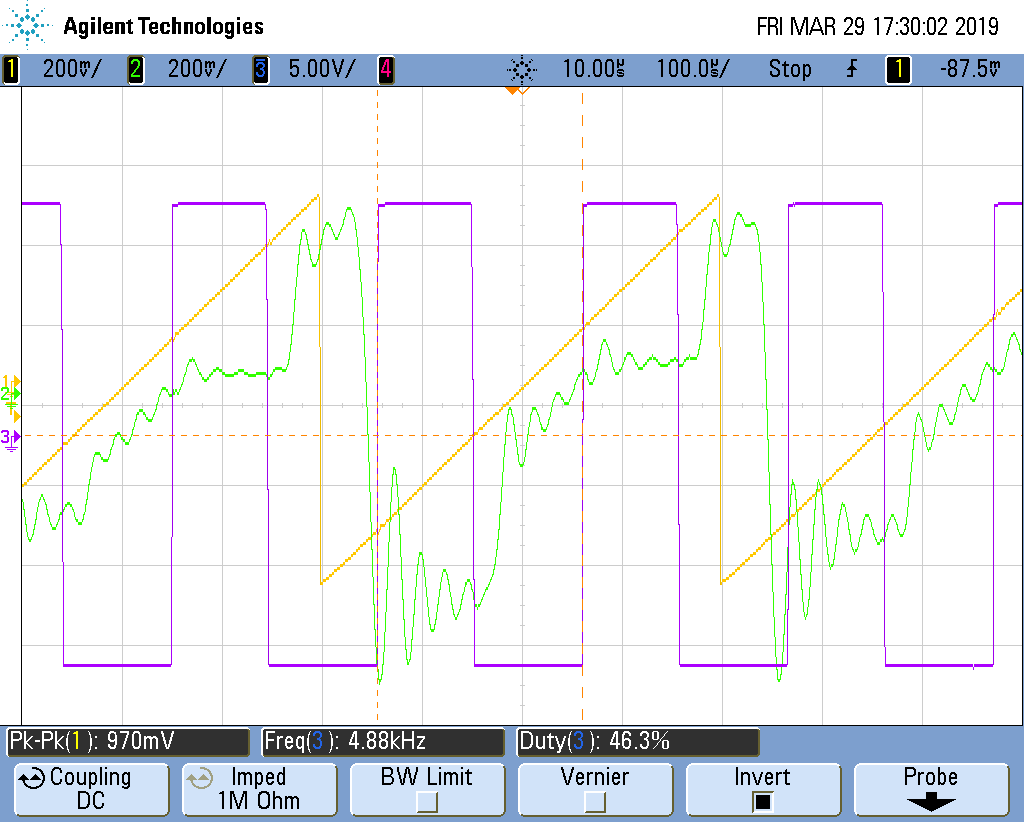
\includegraphics[scale=0.25]{Imagenes/yh_pt6d_cuad2}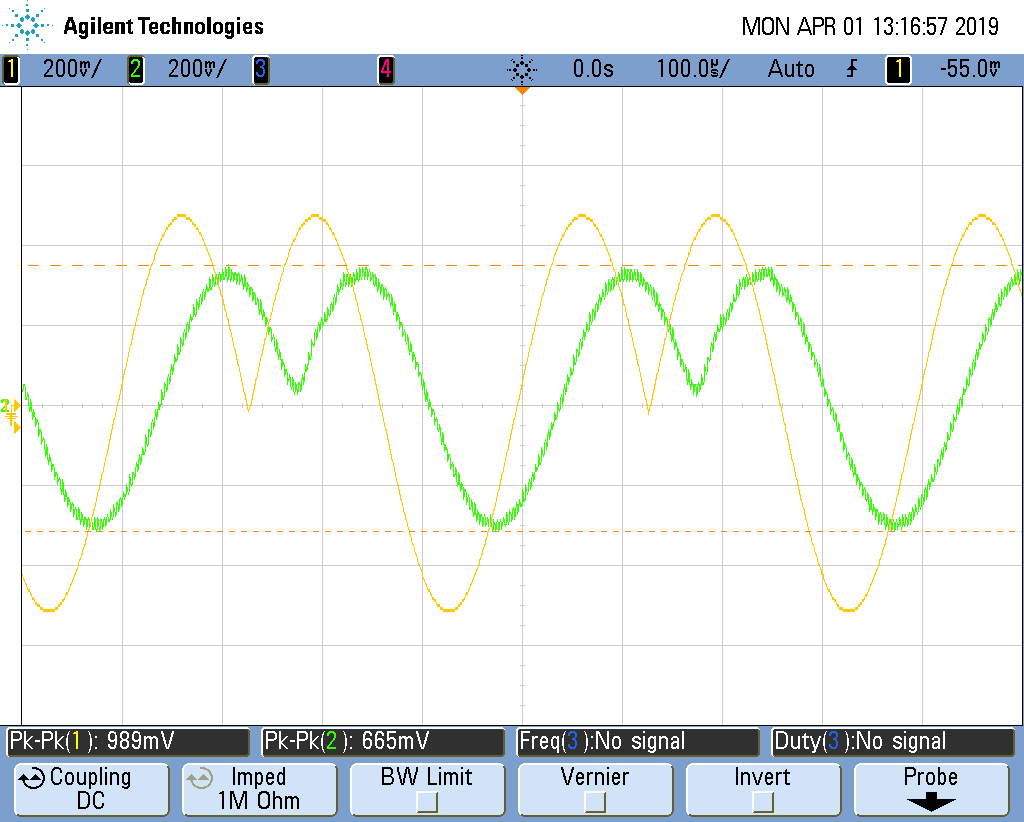
\includegraphics[scale=0.25]{Imagenes/ej_6_d}
\par\end{centering}
\caption{Señal muestreada con una señal de 20kHz.}
\end{figure}

Si ahora simulamos la señal en nuestra GUI, obtenemos lo siguiente:

\begin{figure}[H]
\begin{centering}
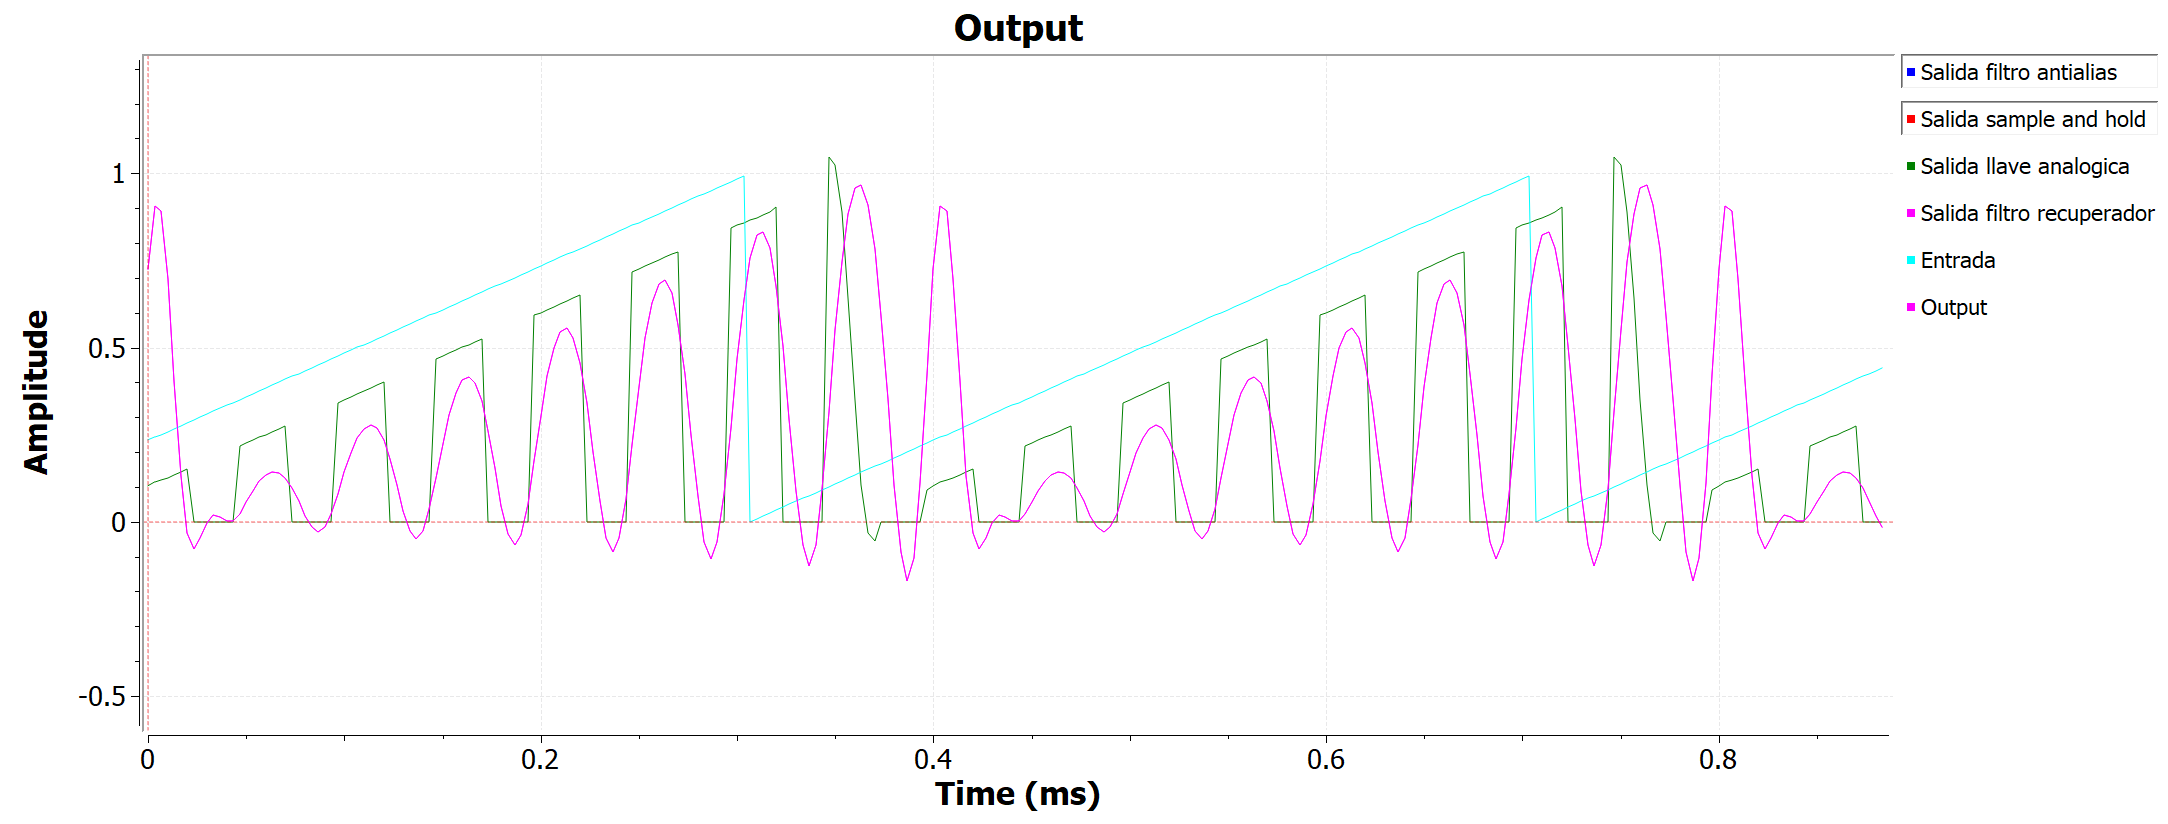
\includegraphics[scale=0.5]{Imagenes/simulacion_llave_diente_d.PNG}
\par\end{centering}
\begin{centering}
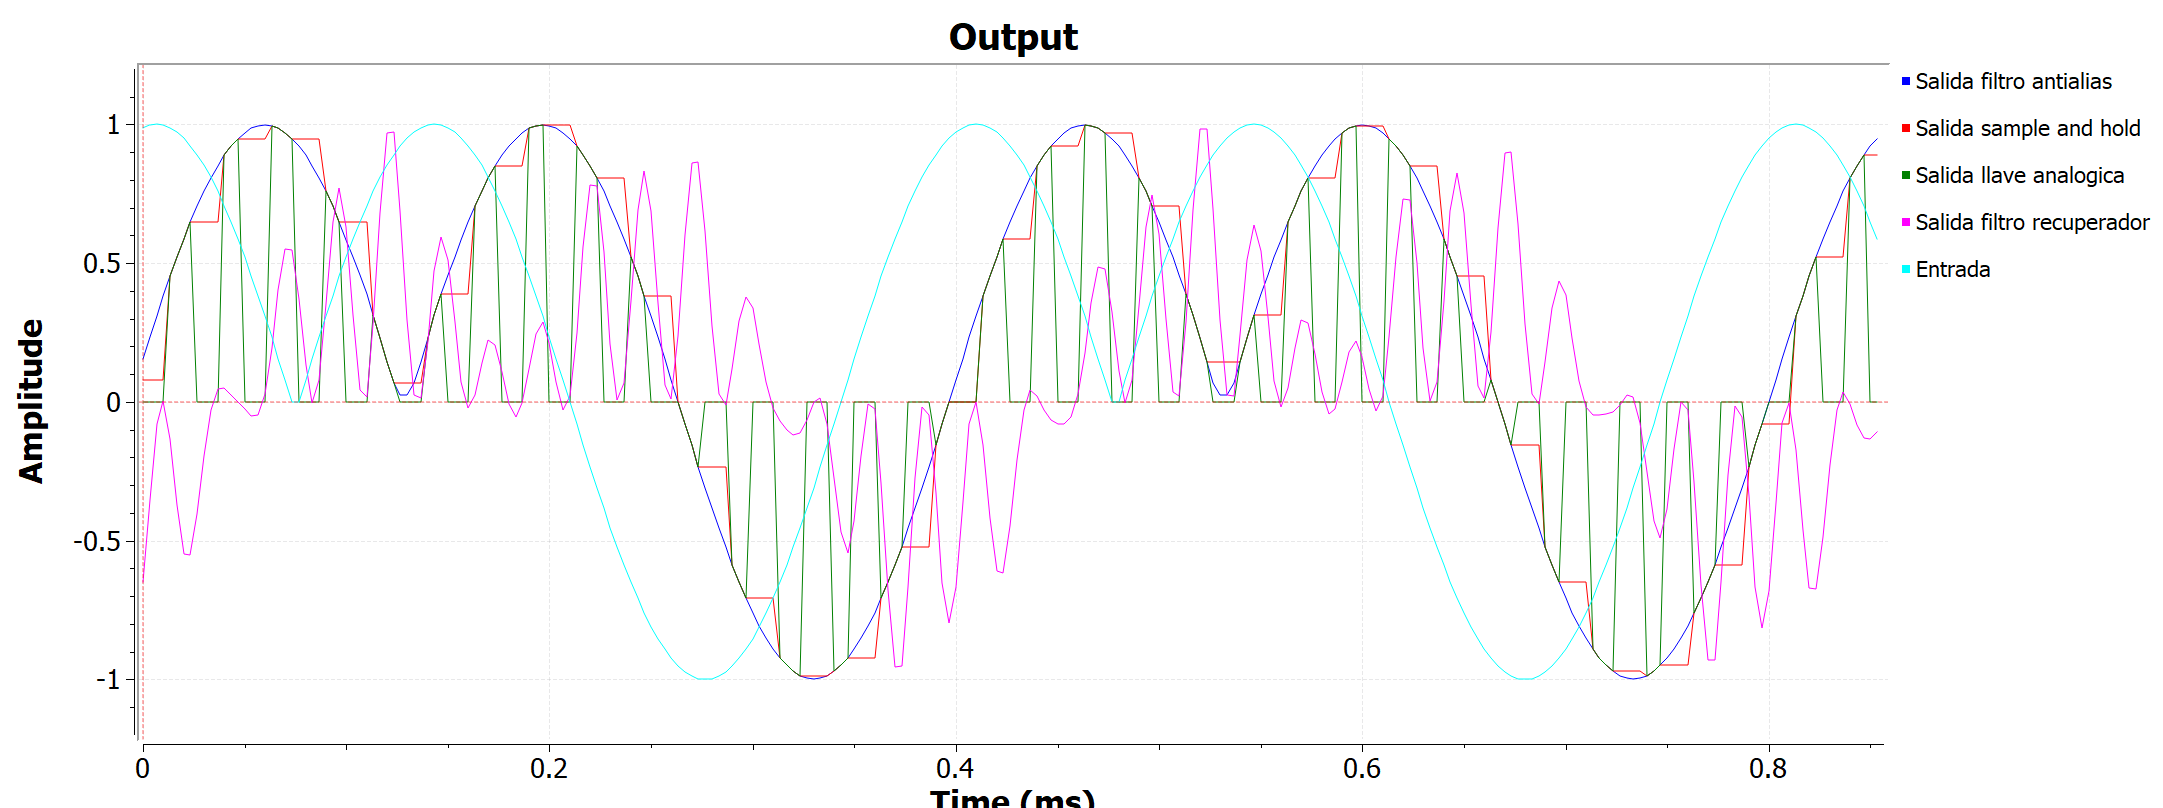
\includegraphics[scale=0.5]{Imagenes/simulacion_llave_senoraro_d.PNG}\caption{Simulación de la señal anterior.}
\par\end{centering}
\end{figure}

Vemos como en la simulación, el efecto de aliasing no aparece en el
rango de frecuencias que se especificaron anteriormente, puesto que
vemos que la salida posee la forma de la señal de entrada. Esto es
el producto de que en la teoría, el muestreo se produce con funciones
$\delta$ , por lo que el espectro de la señal digital queda más disperso
que el que se obtiene en el laboratorio, por lo que a la hora de recuperarlo,
el aliasing se produce a una menor frecuencia $f_{s}$.

\section{Sample and Hold}

\subsection{Optimización}

Similar a la sección 1.1, utilizando el sample and hold , se calibraron
todas las partes de la placa par así poder obtener la menor distorción
posible con un óptimo $f_{s}\,y\,A$. Podemos observar el resultado
en las siguientes imágenes:

\begin{figure}[H]

\begin{centering}
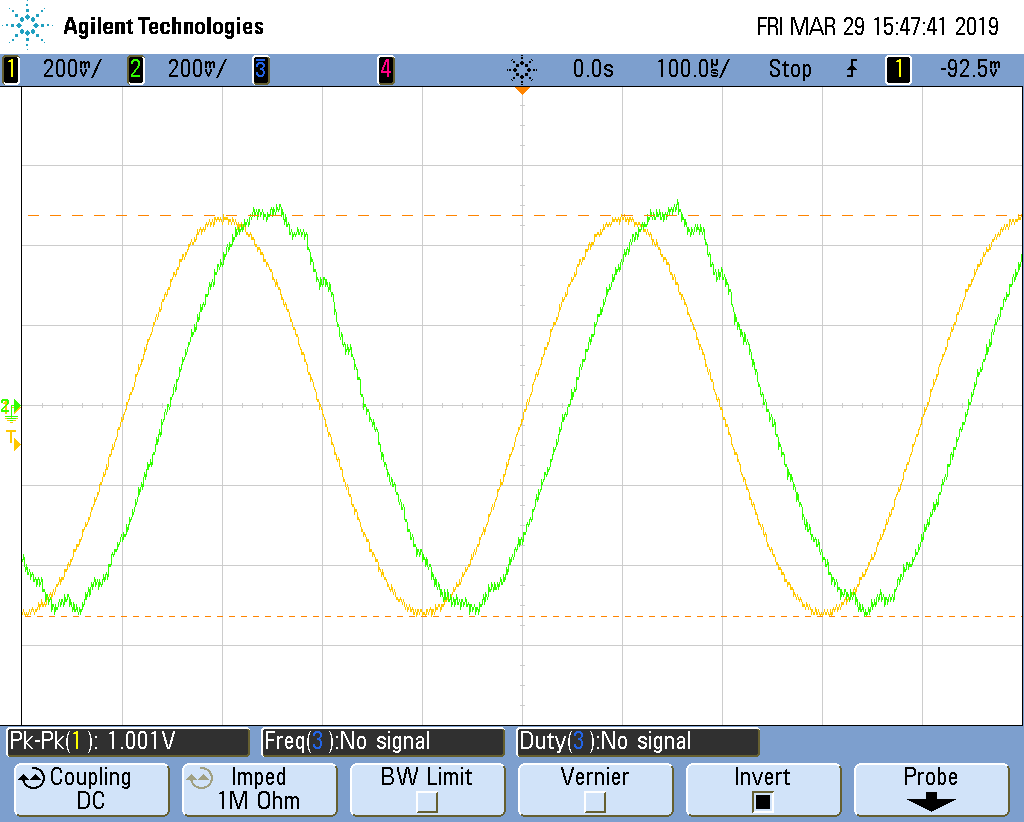
\includegraphics[scale=0.25]{Imagenes/syh_pto_asin3}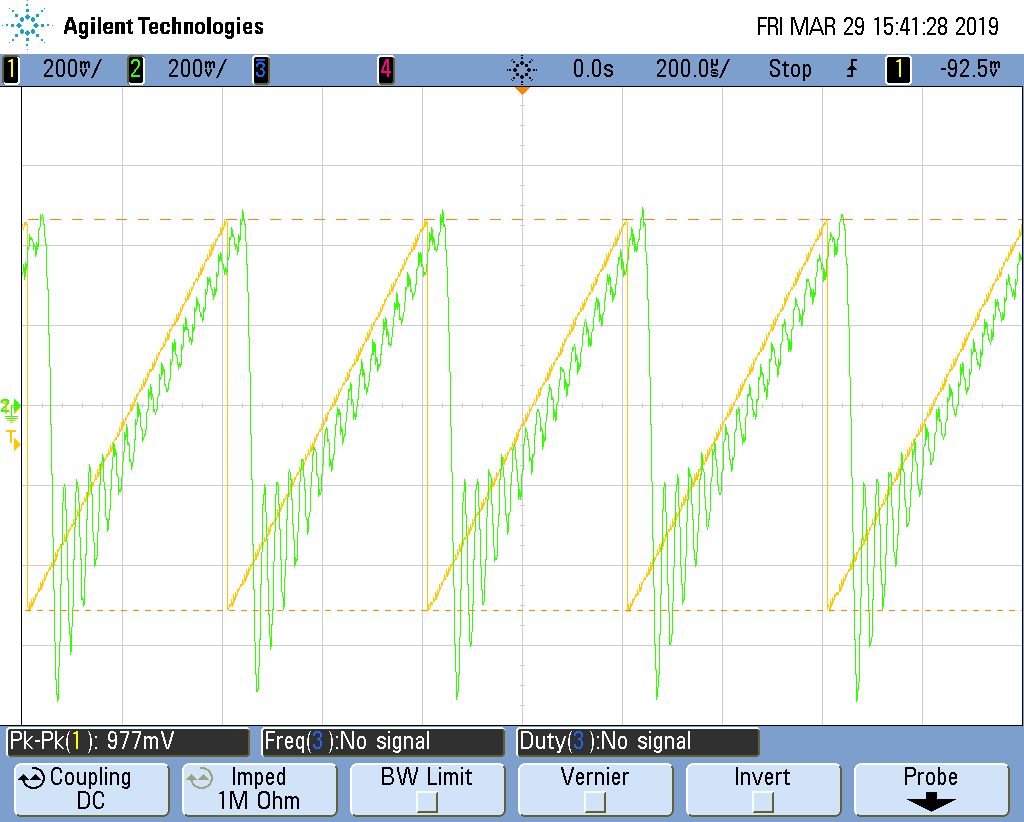
\includegraphics[scale=0.25]{Imagenes/syh_pto_adiente}
\par\end{centering}
\centering{}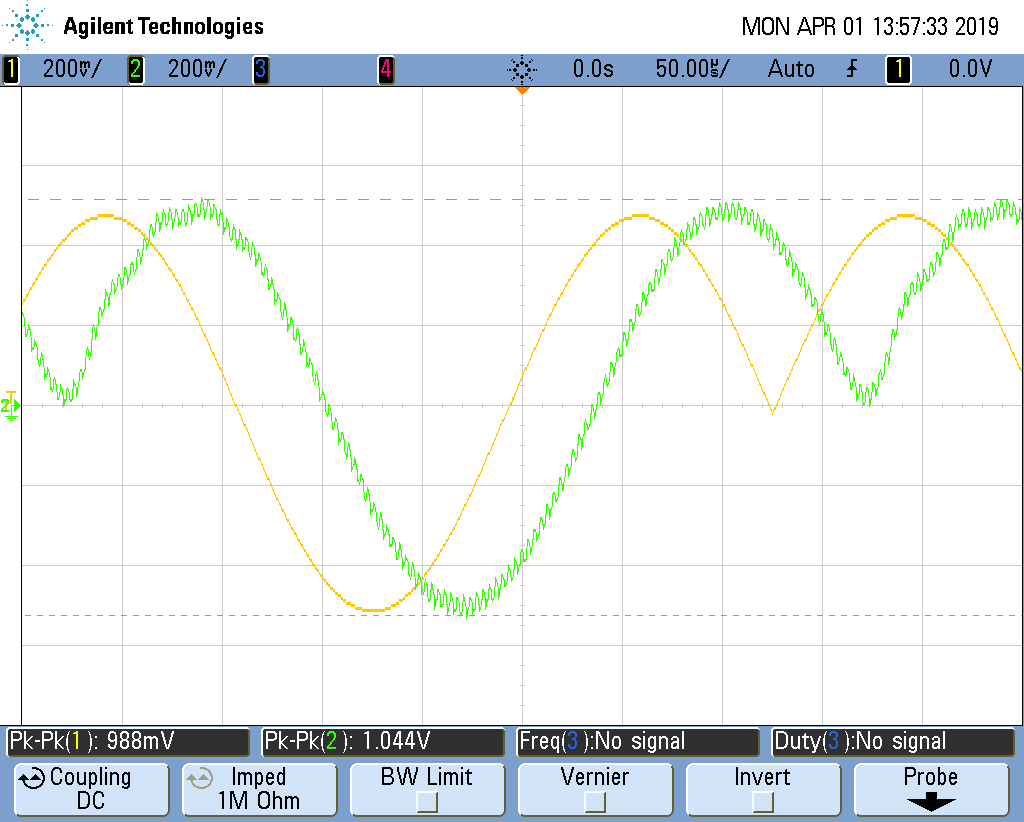
\includegraphics[scale=0.25]{Imagenes/ej_6_a_syh}\caption{De izq a der: salida (verde) de la placa con $X_{a}$; salida con
$X_{b}$}
\end{figure}

Para la señal $X_{a}$, los valores óptimos que se obtuvieron fueron:
$f_{s}:[83;307](kHz)$midiendo en el máximo de ese intervalo, $DC=34.5\%,$$A:(0;2]$(Vpp)
midiendo para $A=1V_{pp}$.

Para la señal $X_{b}$, los valores óptimos obtenidos fueron: $f_{s}:[91;307](kHz)$
midiendo en la frecuencia de 290kHz (pertenceciente a ese intervalo),
$DC=[30;47.5](\%)$, $A:(0;2]$(Vpp) midiendo para $A=1V_{pp}$.

Para la señal $X_{c}$, los valores óptimos obtenidos fueron: $f_{s}:[51;313](kHz)$midiendo
en el máximo de ese intervalo, $DC=48\%,$$A:(0;2]$(Vpp) midiendo
para $A=1V_{pp}$.

Utilizando el entorno de simulación realizado, obtuvimos las siguientes
imagenes:

\begin{figure}[H]

\begin{centering}
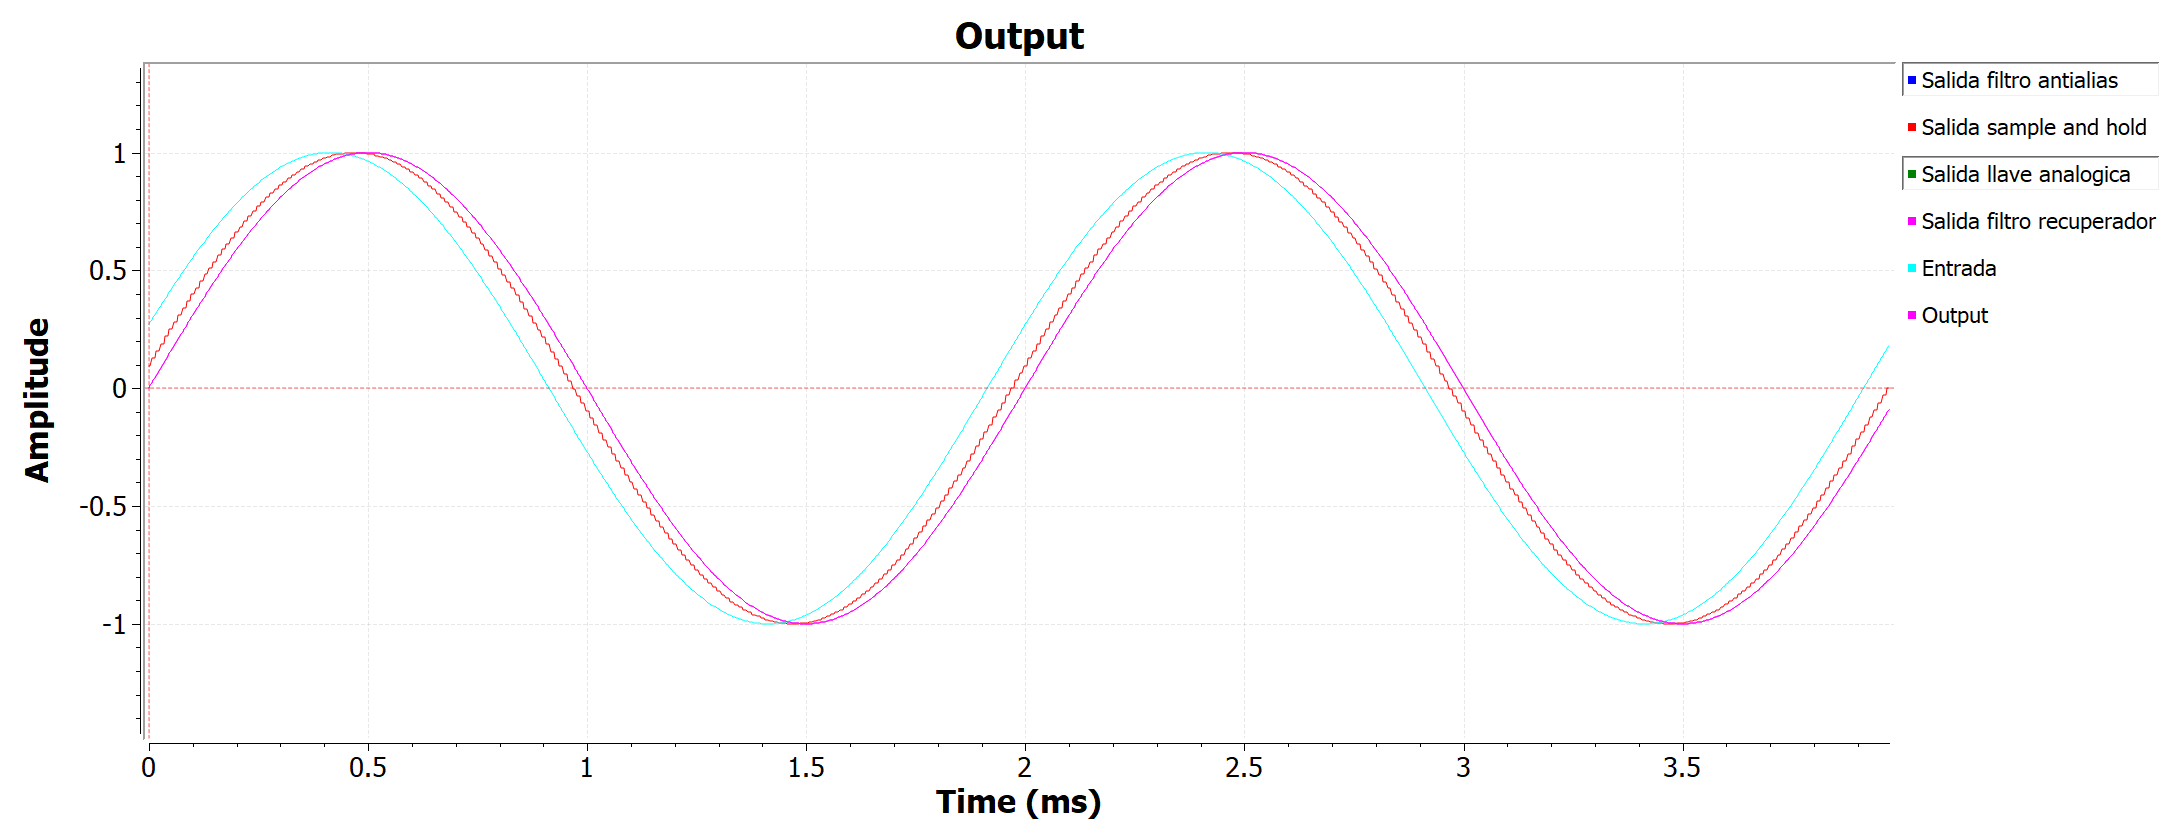
\includegraphics[scale=0.5]{Imagenes/simulacion_syh_seno_a.PNG}
\par\end{centering}
\begin{centering}
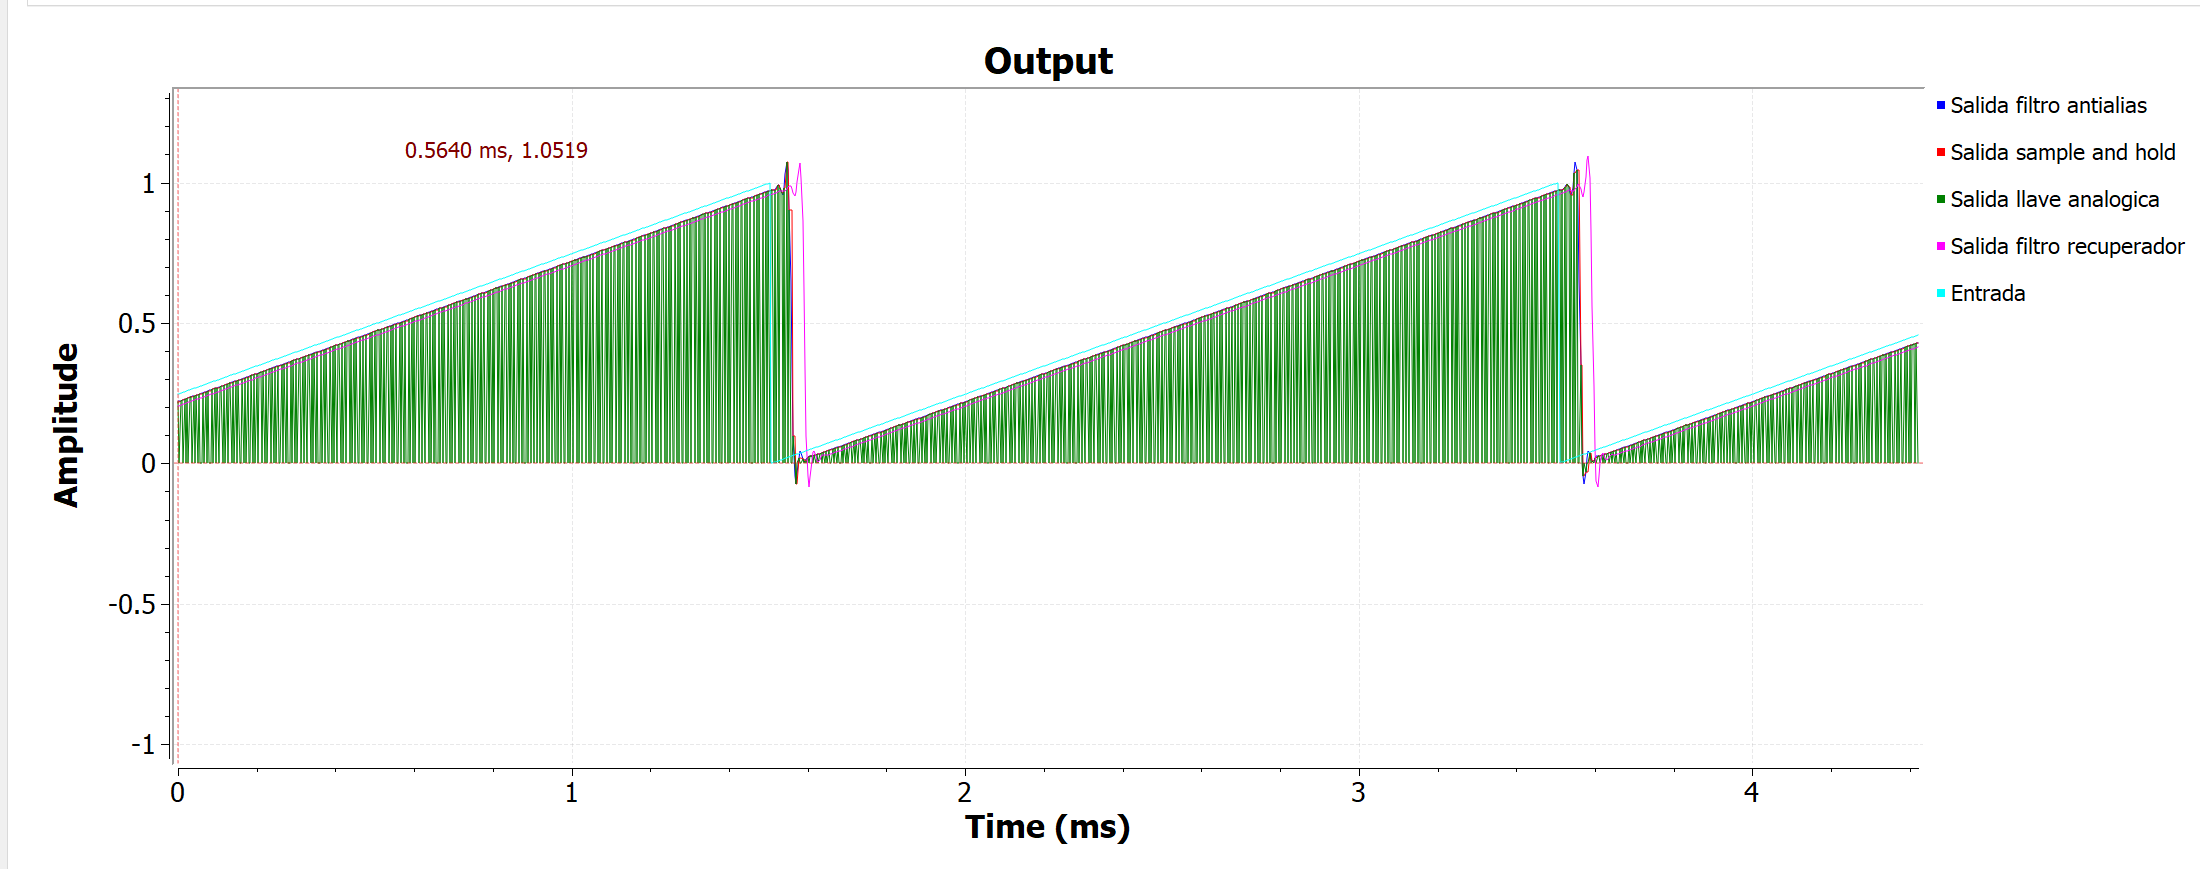
\includegraphics[scale=0.5]{Imagenes/simulacion_syh_diente_a.PNG}
\par\end{centering}
\begin{centering}
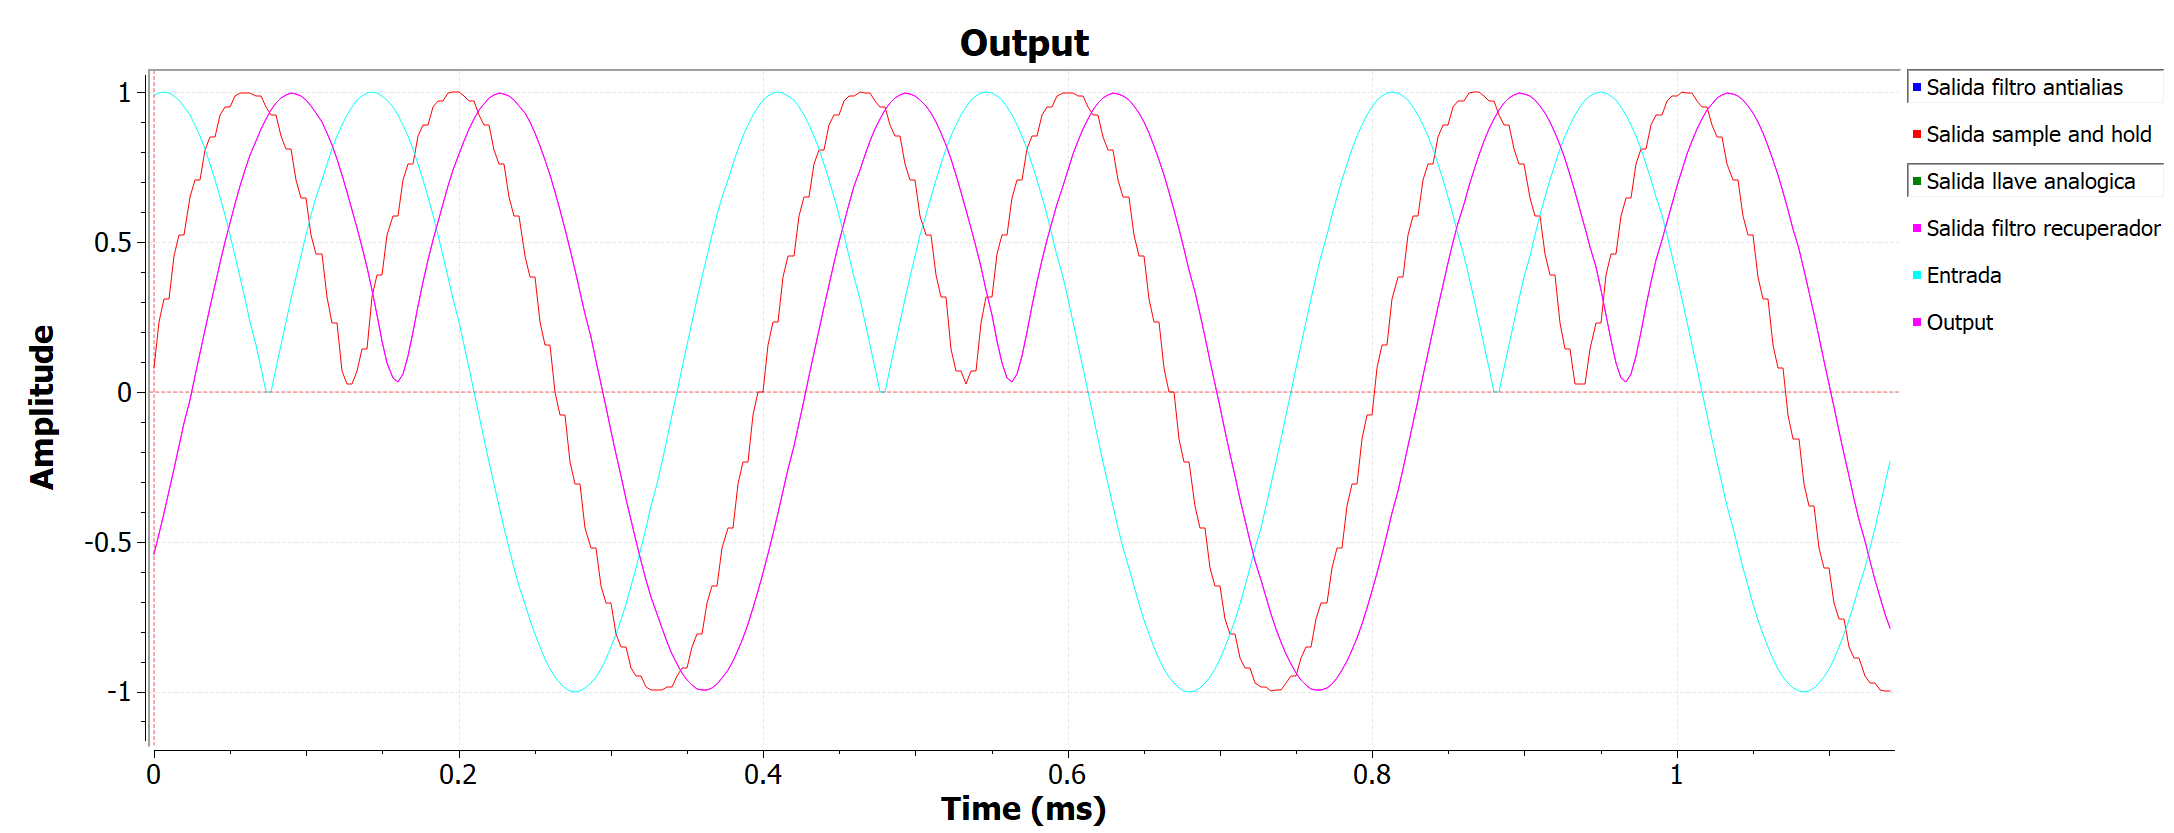
\includegraphics[scale=0.5]{Imagenes/simulacion_syh_senoraro_a.PNG}\caption{Simulaciones realizadas en el GUI.}
\par\end{centering}
\end{figure}

Podemos ver como lo obtenido en las mediciones no discrepan con las
simulaciones. Si acaso podemos destacar que para la función rampa
simulada no se aprecia un ripple montado sobre sí, lo cual puede ser
explicado desde las falencias de nuestro filtro mencionadas previamente
en este trabajo práctico.

\subsection{Cambios en la $f_{in}$ y en la $f_{s}$}

\subsubsection{$f_{in}<\frac{f_{p}}{2}$,$f_{s}=f_{a}$}

Para este caso, se exitó a la placa con una señal $X_{a}$, con la
diferencia respecto al punto anterior de que ahora el rango de $f_{in}=(0;17.5]$(kHz)
y la $f_{s}=68kHz.$Con el nuevo intervalo de $f_{in}$, finalmente
se eligió $f_{in}=500Hz.$ El duty cycle utilizado fue de 47.6\%.

Para la señal $X_{b}$, por otra parte el rango de $f_{in}$ pasó
a ser $f_{in}=(0;11.5]$(kHz) y la $f_{s}$ mantuvo su valor de $68kHz.$Con
el nuevo intervalo de $f_{in}$, finalmente se eligió $f_{in}=11.5kHz.$
El duty cycle utilizado también fue de 47.6\%.

Por último para la señal $X_{c}$, el rango de $f_{in}$ pasó a ser
$f_{in}=(0;0.5]$(kHz) mientras que la $f_{s}$ mantuvo su valor de
$68kHz.$Con el nuevo intervalo de $f_{in}$, finalmente se eligió
$f_{in}=500Hz.$ El duty cycle utilizado también fue de 49.8\%.

Los resultados se ven plasmados en la siguiente image:

\begin{figure}[H]

\begin{centering}
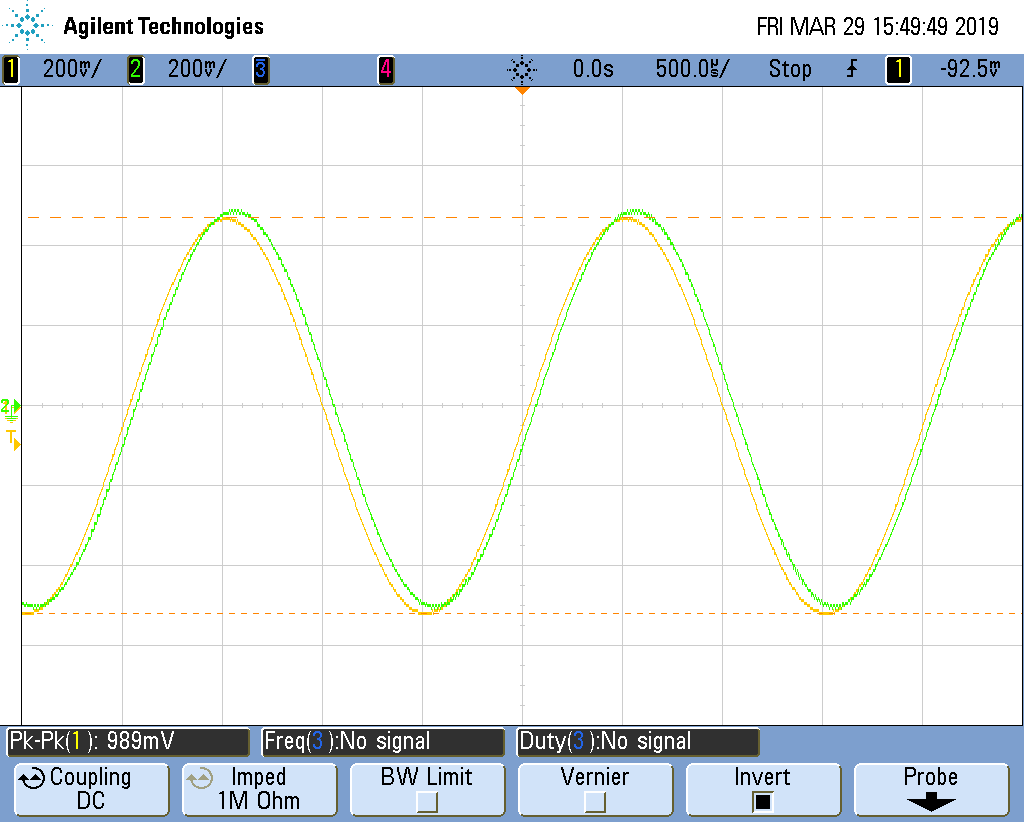
\includegraphics[scale=0.25]{Imagenes/syh_pto_bsin}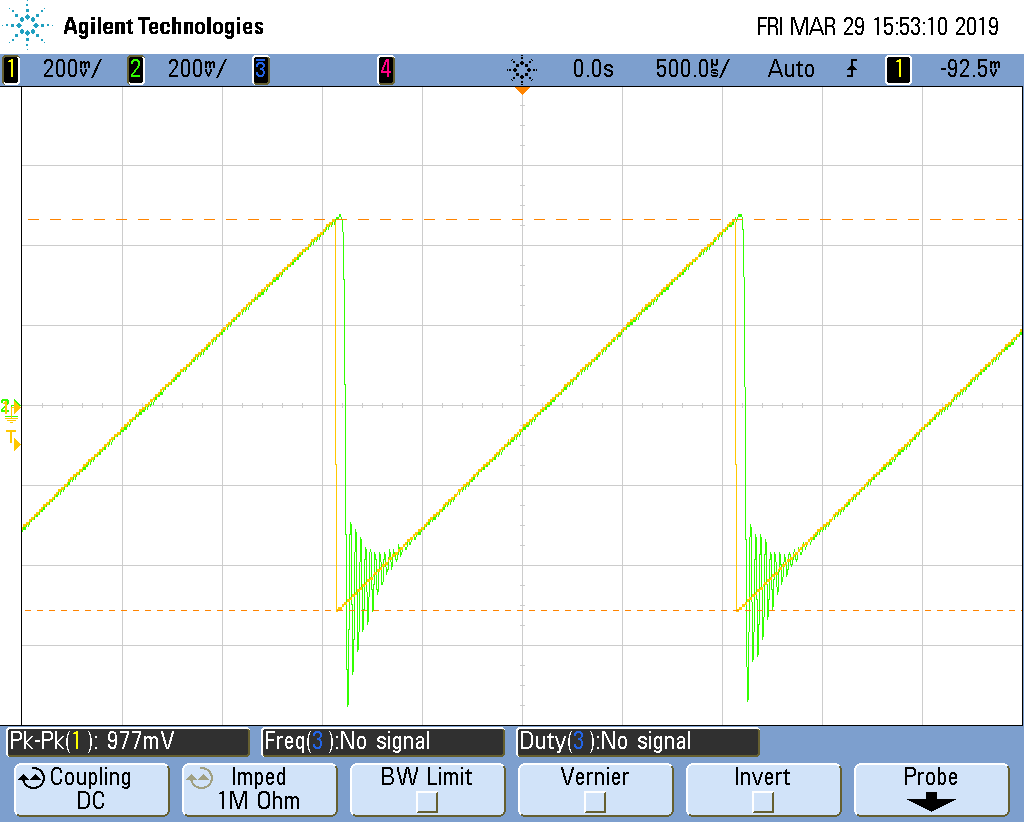
\includegraphics[scale=0.25]{Imagenes/syh_pto_bcuad_1}
\par\end{centering}
\begin{centering}
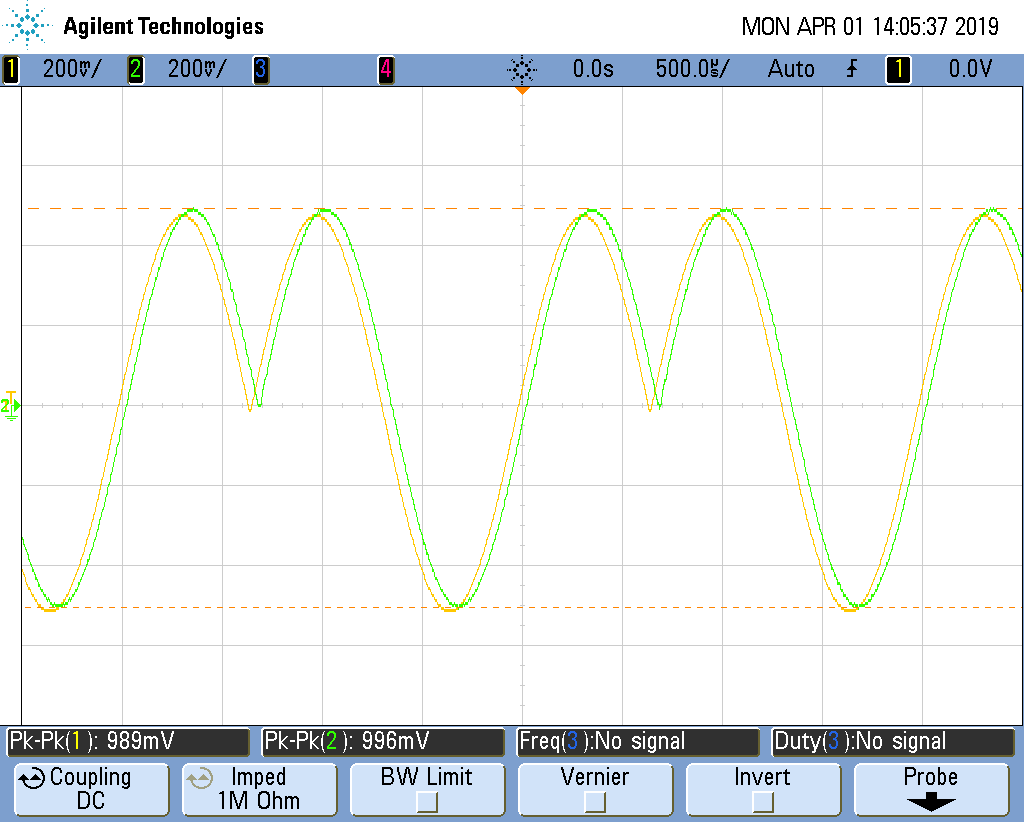
\includegraphics[scale=0.25]{Imagenes/ej_6_b_syh}\caption{De izquierda a derecha: señal $X_{a}$y señal $X_{b}$.}
\par\end{centering}
\end{figure}

Ahora, simulando lo previamente relatado, podemos ver una diferencia
entre la función rampa obtenida en el osciloscopio y la simulada:
vemos que en osciloscopio podemos recuperar la señal de manera cuasi
perfecta a exepción del ripple que nos aparece al principio; pero
si observamos la simulación vemos que la señal de salida presenta
un menor contenido armónico.

\begin{figure}[H]

\begin{centering}
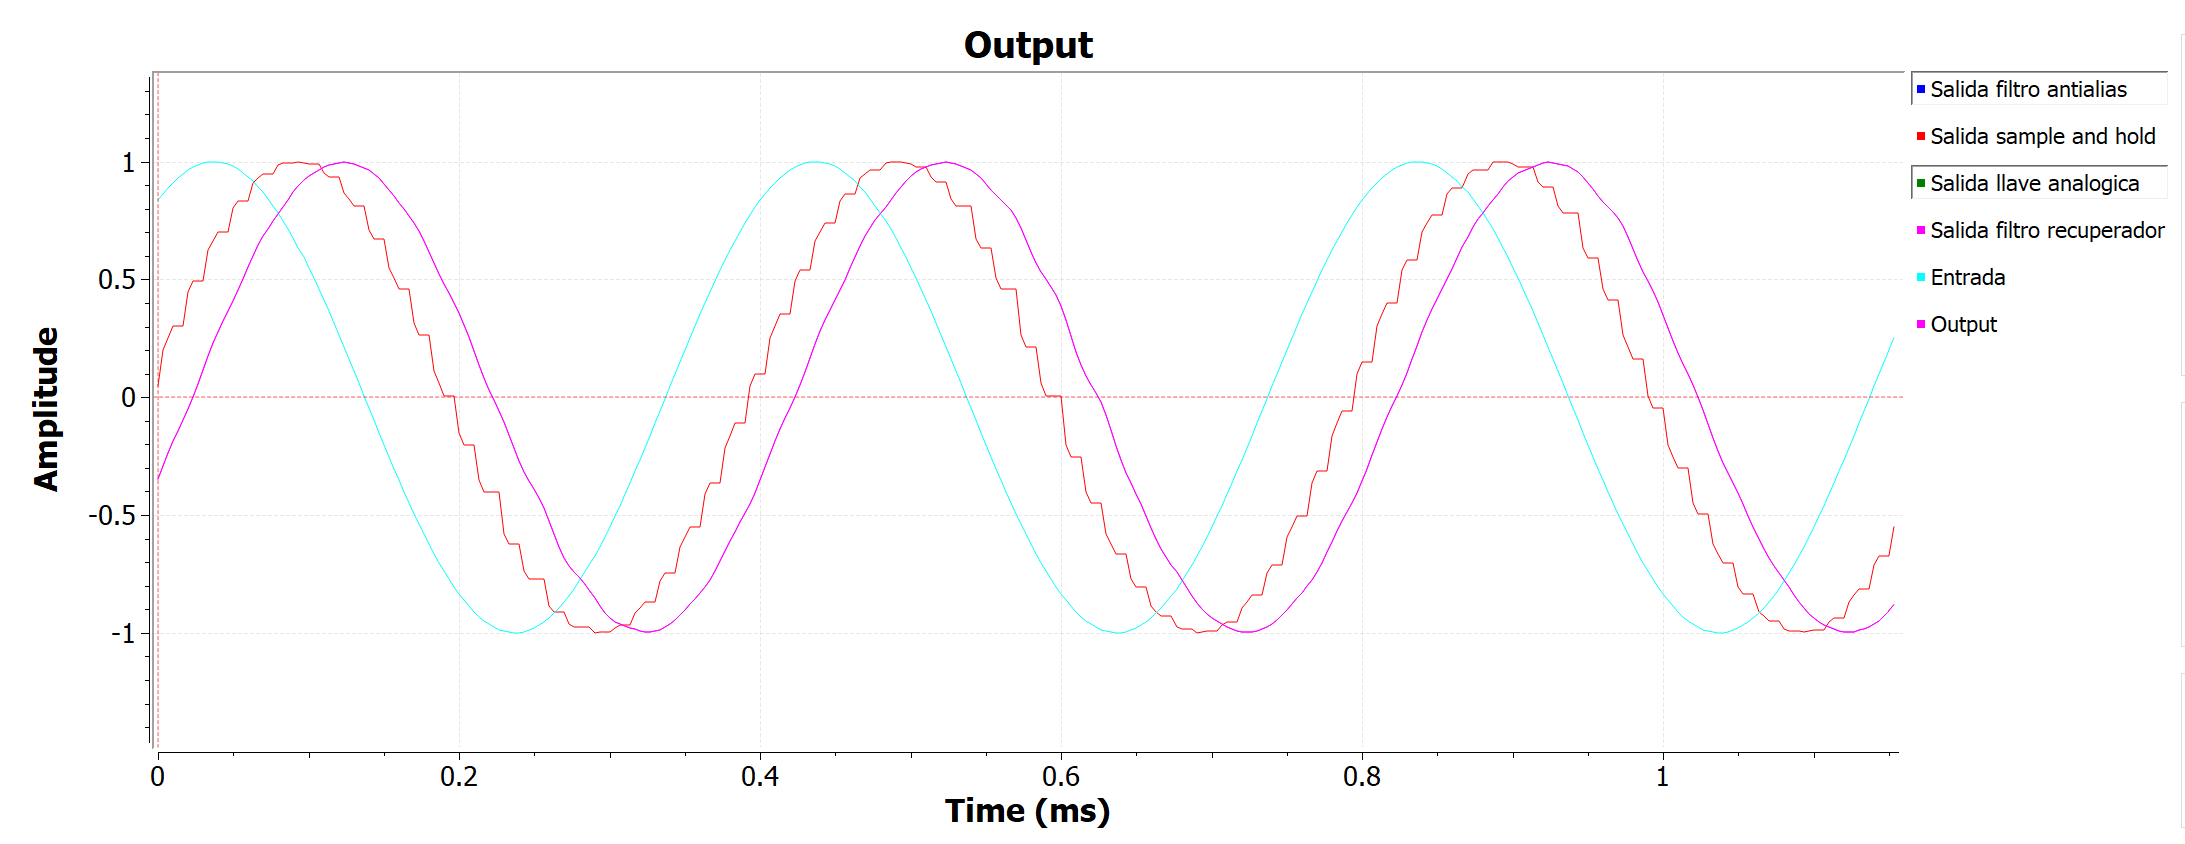
\includegraphics[scale=0.5]{Imagenes/simulacion_syh_seno_b1.PNG}
\par\end{centering}
\begin{centering}
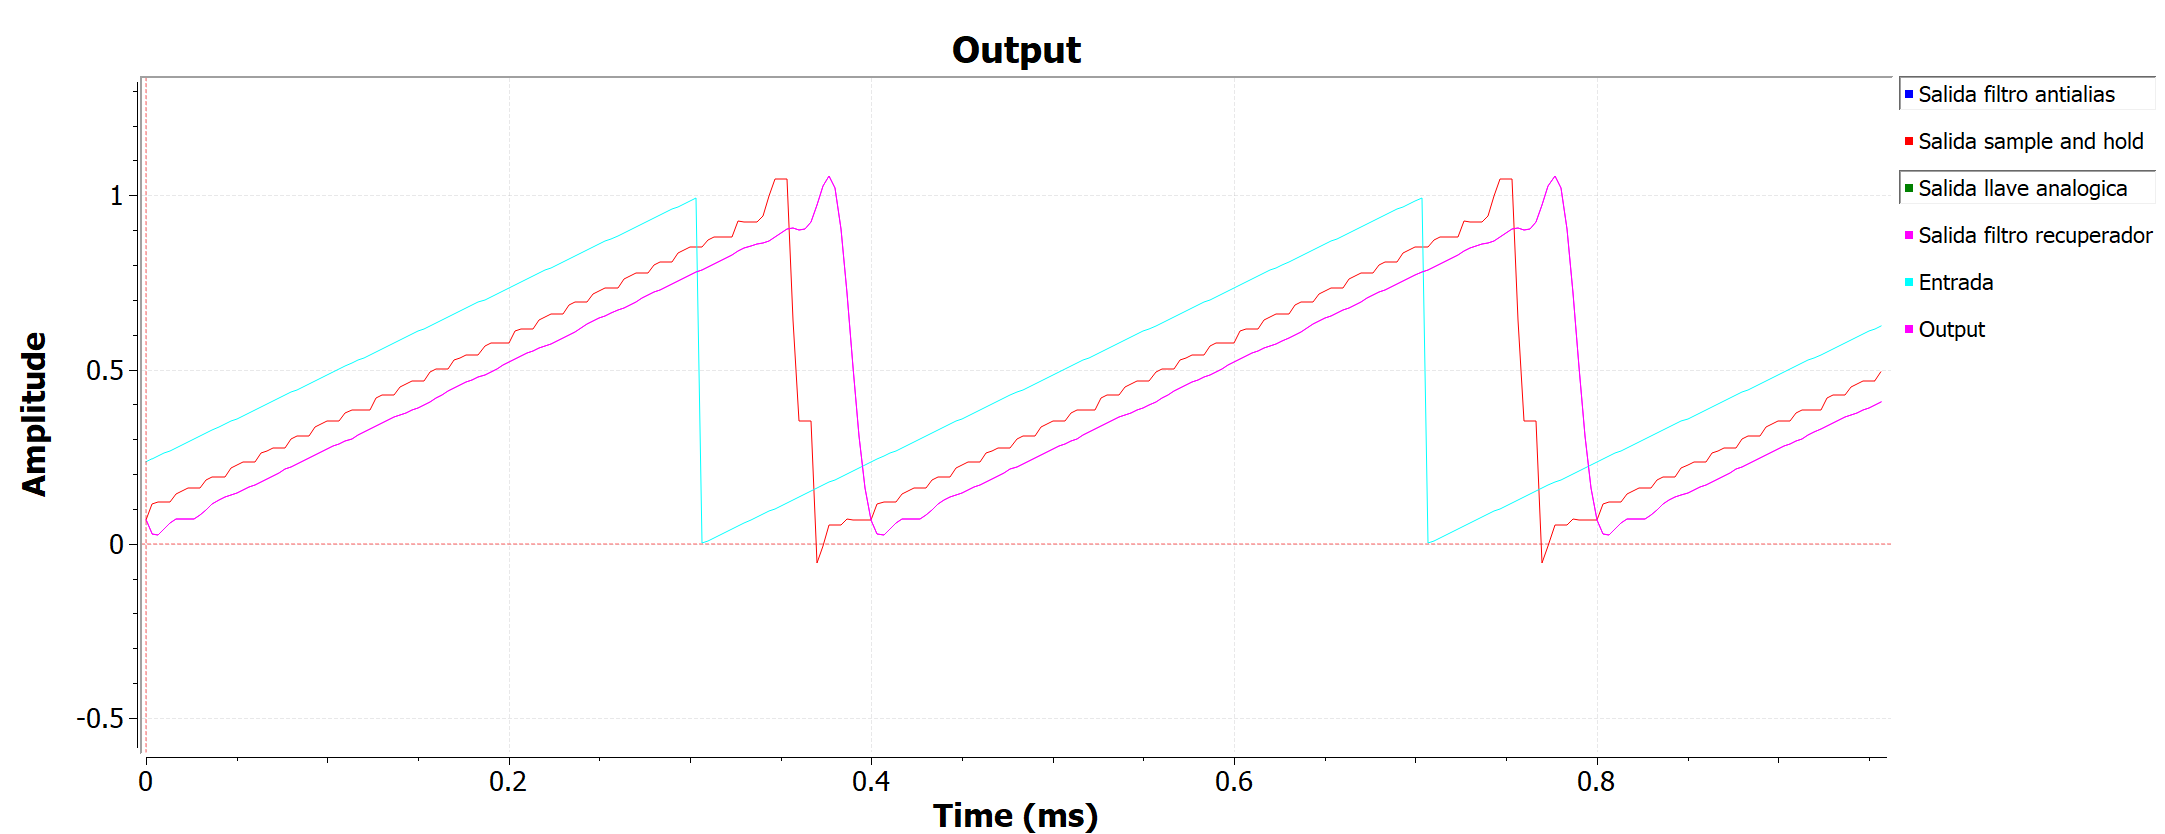
\includegraphics[scale=0.5]{Imagenes/simulacion_syh_diente_b1.PNG}\caption{De izquierda a derecha: señal $X_{a}$y señal $X_{b}$simuladas.}
\par\end{centering}
\end{figure}


\subsubsection{$f_{in}=f_{a}$}

Para este punto, nuevamente, tanto a la señal $X_{a}$ como $X_{b}$,
se las estableció con una frecuencia $f_{in}=68kHz$. Para la frecuencia
de muestreo, se optó por utilizar la máxima posible, es decir $f_{s}=313kHz.$Para
ambas señales, se mantuvo el mismo duty cycle de 48\%. Los resultados
pueden ser apreciados en la siguiente imagen:

\begin{figure}[H]

\begin{centering}
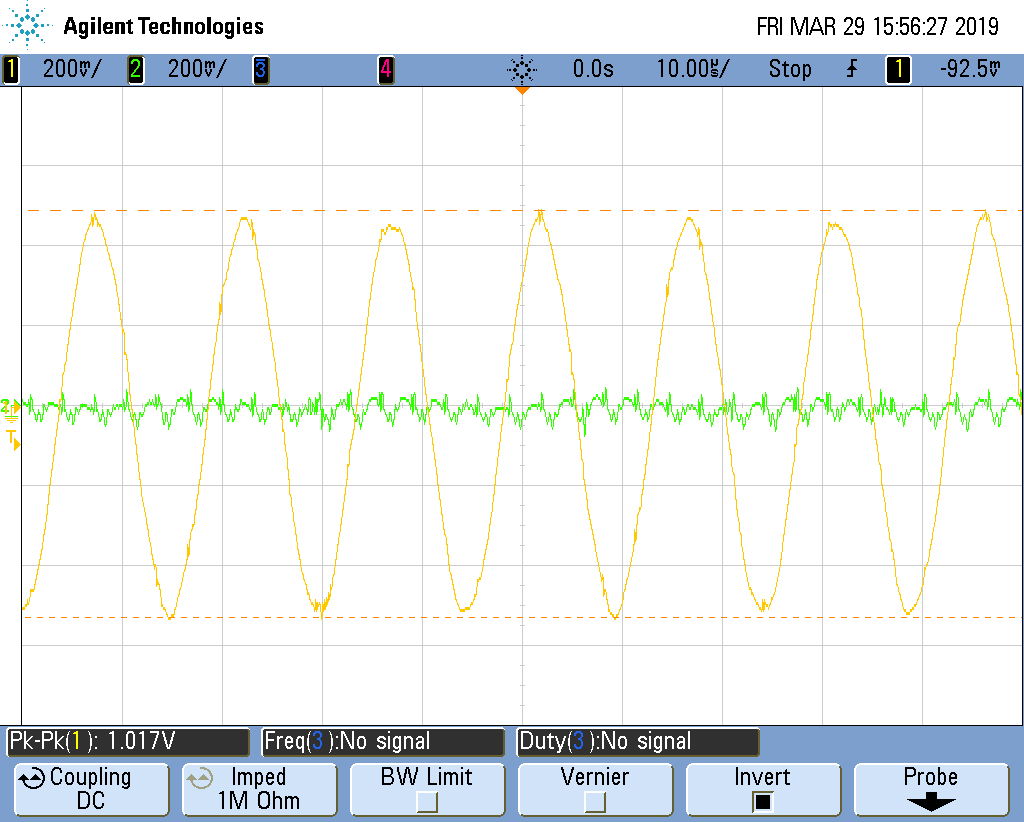
\includegraphics[scale=0.25]{Imagenes/syh_pto_bsin_67k}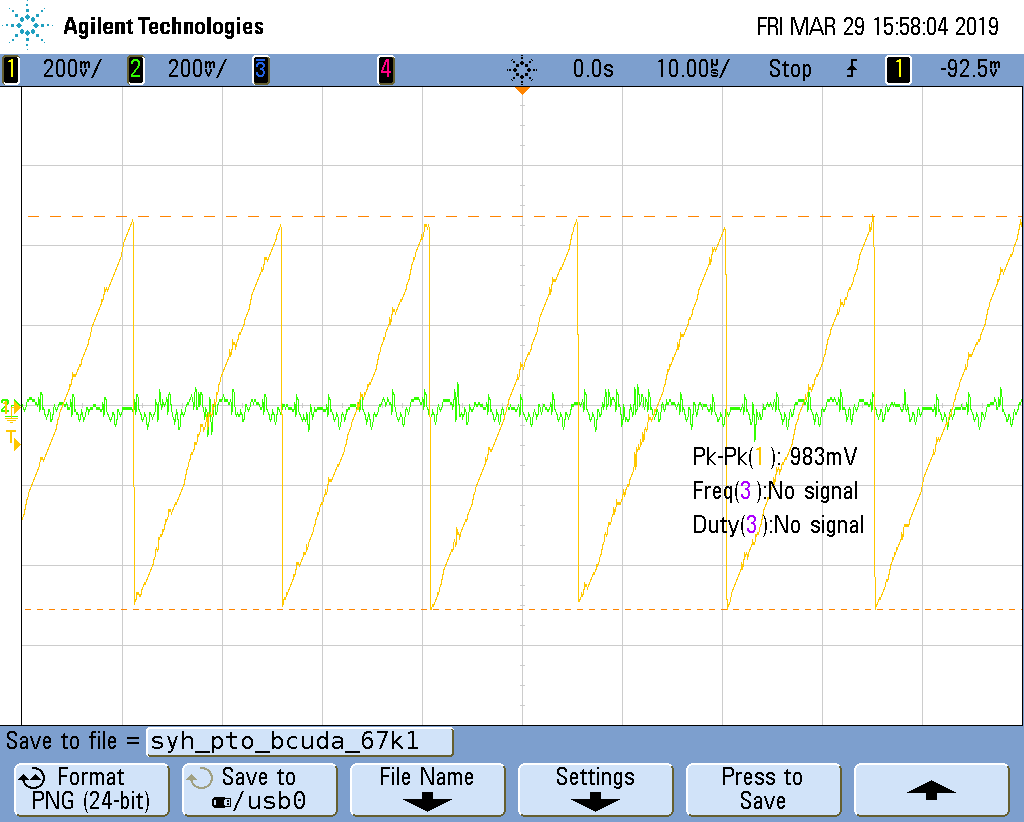
\includegraphics[scale=0.25]{Imagenes/syh_pto_bcuda_67k1}
\par\end{centering}
\begin{centering}
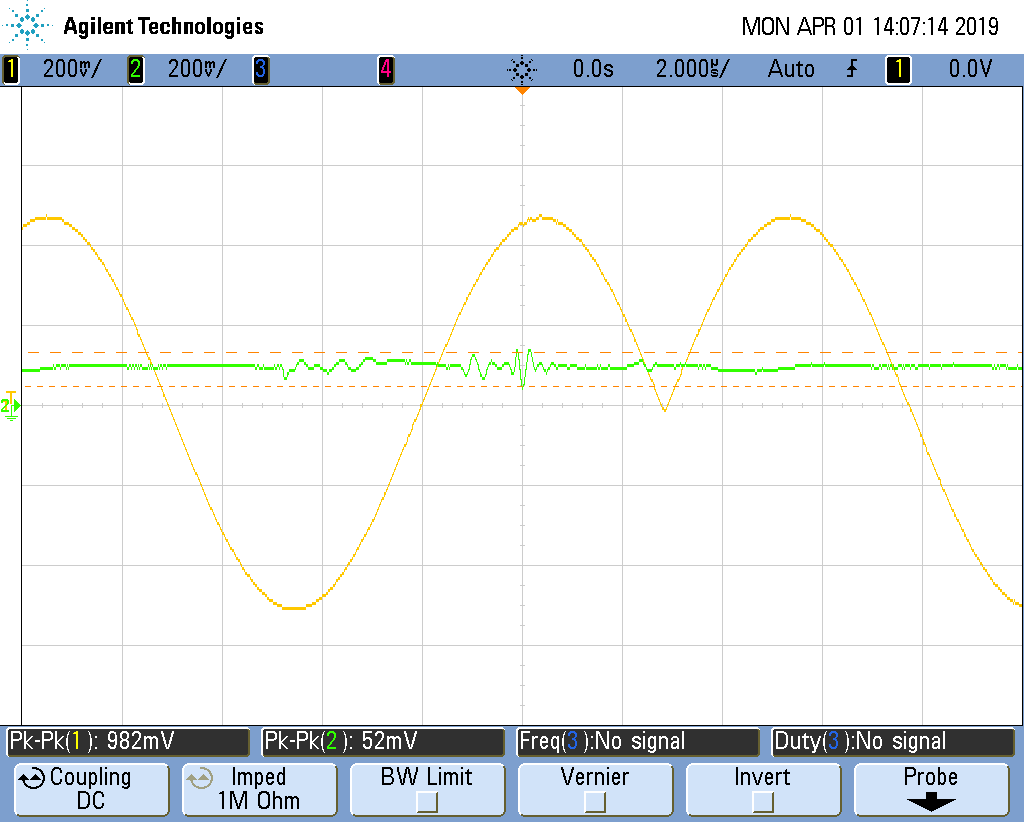
\includegraphics[scale=0.25]{Imagenes/ej_6_b_syh2}\caption{De izquierda a derecha: señal $X_{a}$y señal $X_{b}$.}
\par\end{centering}
\end{figure}

Ahora, simulando, obtenemos lo siguiente:

\begin{figure}[H]

\begin{centering}
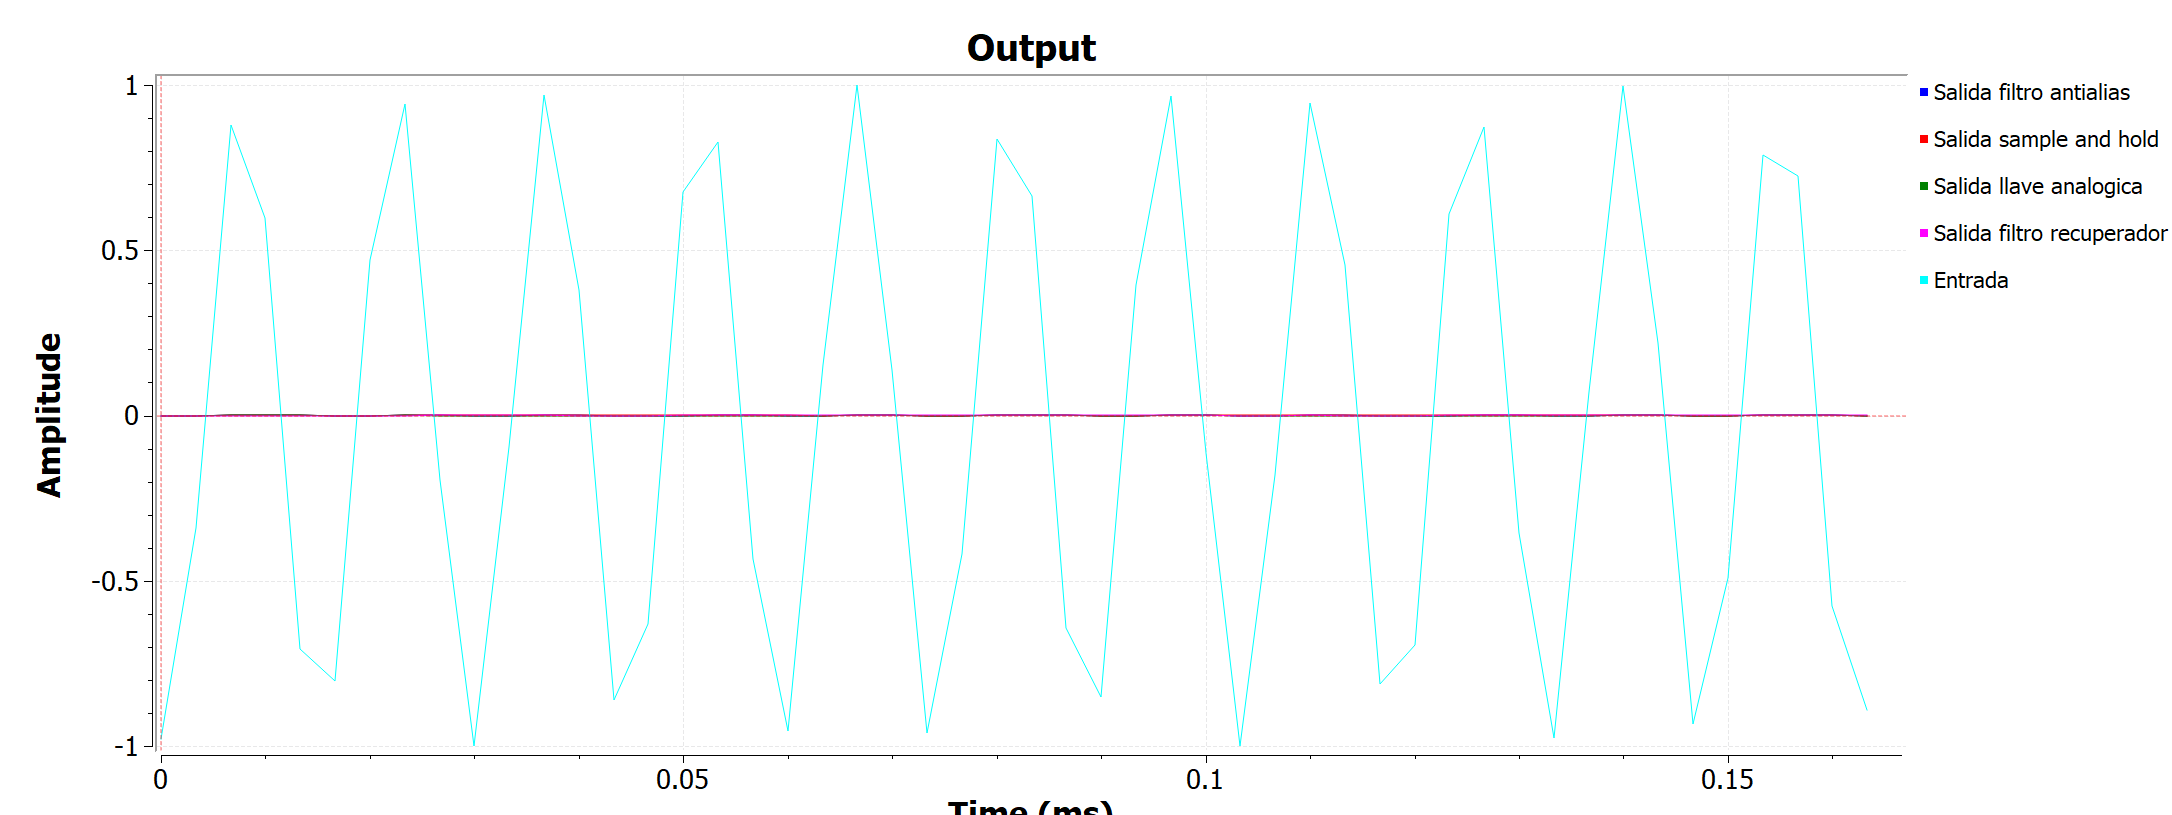
\includegraphics[scale=0.5]{Imagenes/simulacion_syh_seno_b2.PNG}
\par\end{centering}
\begin{centering}
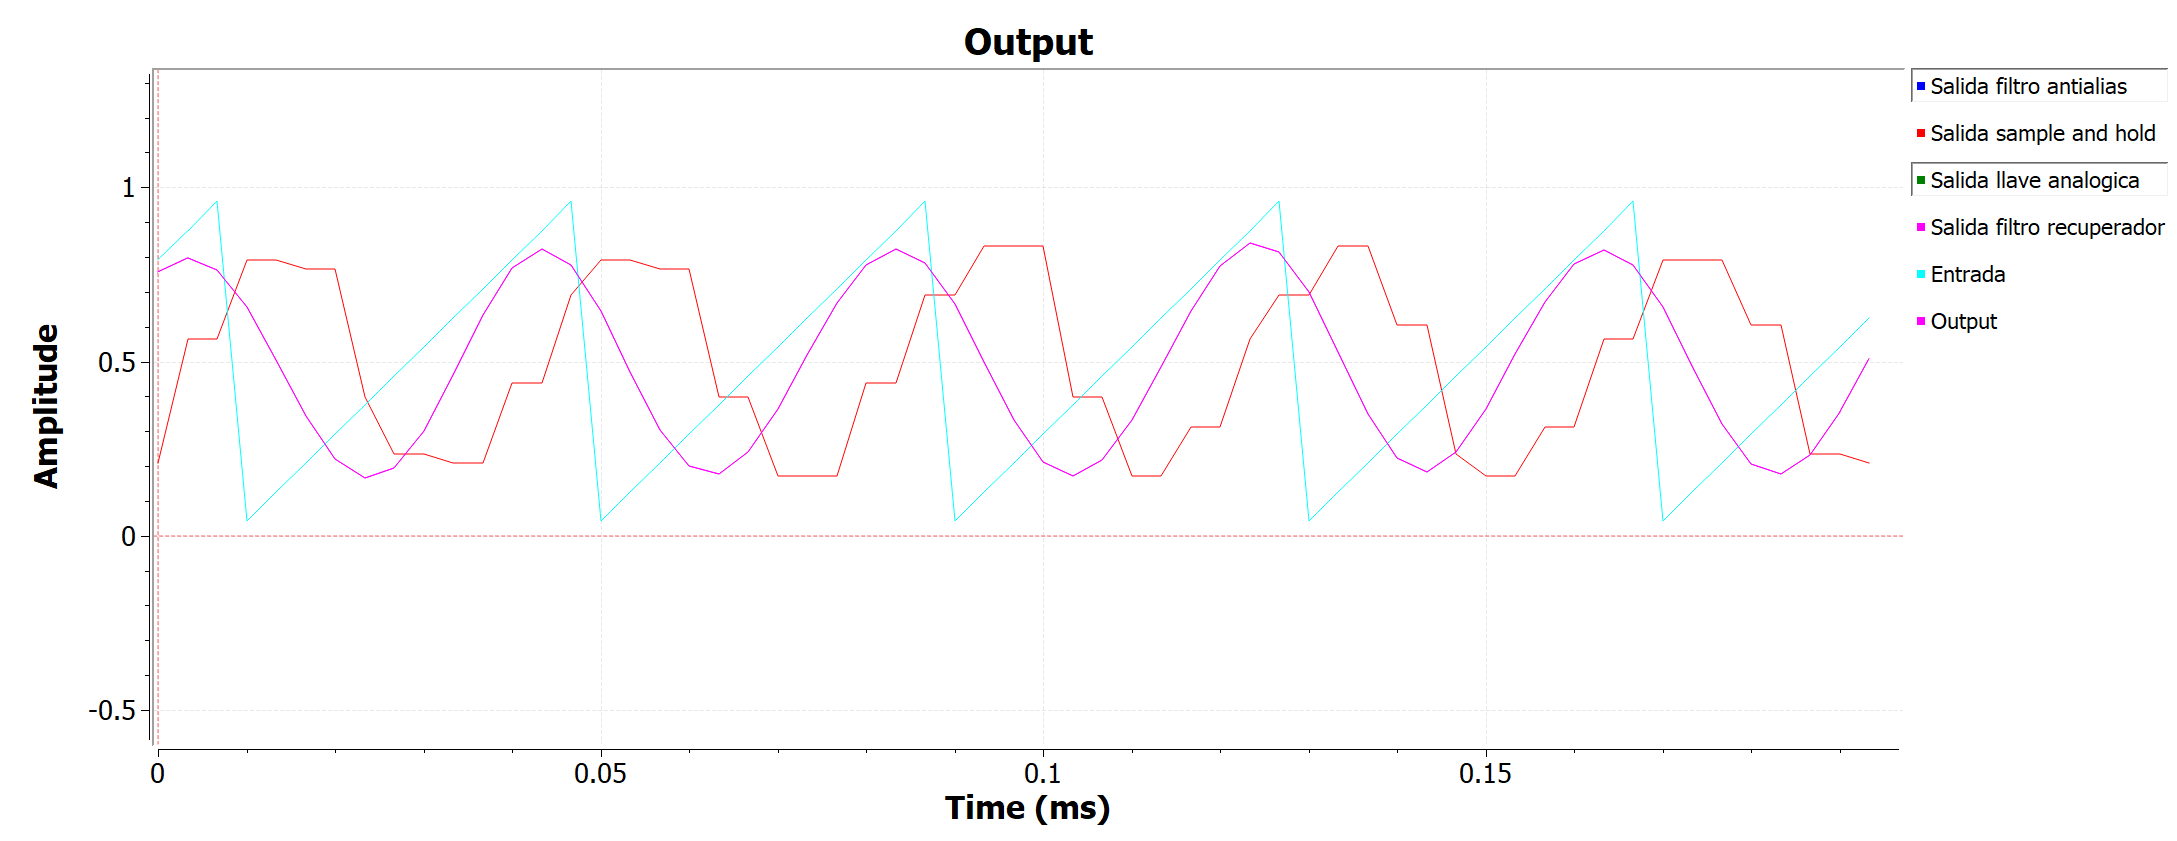
\includegraphics[scale=0.5]{Imagenes/simulacion_syh_diente_b2.PNG}\caption{De izquierda a derecha: señal $X_{a}$y señal $X_{b}$ simuladas.}
\par\end{centering}
\end{figure}

Vemos como efectivamente la señal es nula y totalmente deformada en
ambos casos.

\subsection{$f_{in}=f_{s}\protect\leq f_{p}$}

Para este caso, igual que para su par con llave analógica, solamente
se exito al circuito con la señal $X_{a}$ con la particularidad que
la frecuencia de la señal coincide con la frecuencia de sampleo. Para
ello, se optó por utilizar $f_{in}=f_{s}=10kHz$ y un DC de 47.1\%.
La salida resultante se aprecia a continuación:

\begin{figure}[H]

\begin{centering}
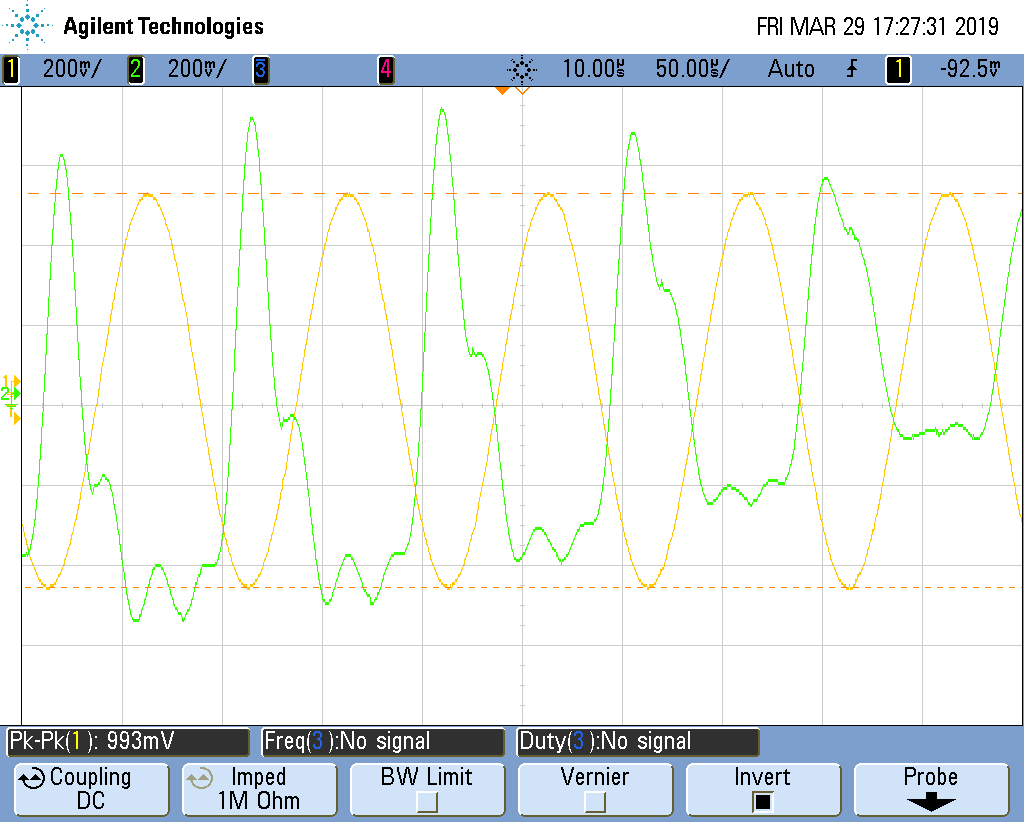
\includegraphics[scale=0.3]{Imagenes/yh_pt6c_sin2}\caption{Señal $X_{b}$ con frecuencia de muestreo igual a la de la señal.}
\par\end{centering}
\end{figure}

Ahora simulando el caso en la GUI, obtenemos:

\begin{figure}[H]
\begin{centering}
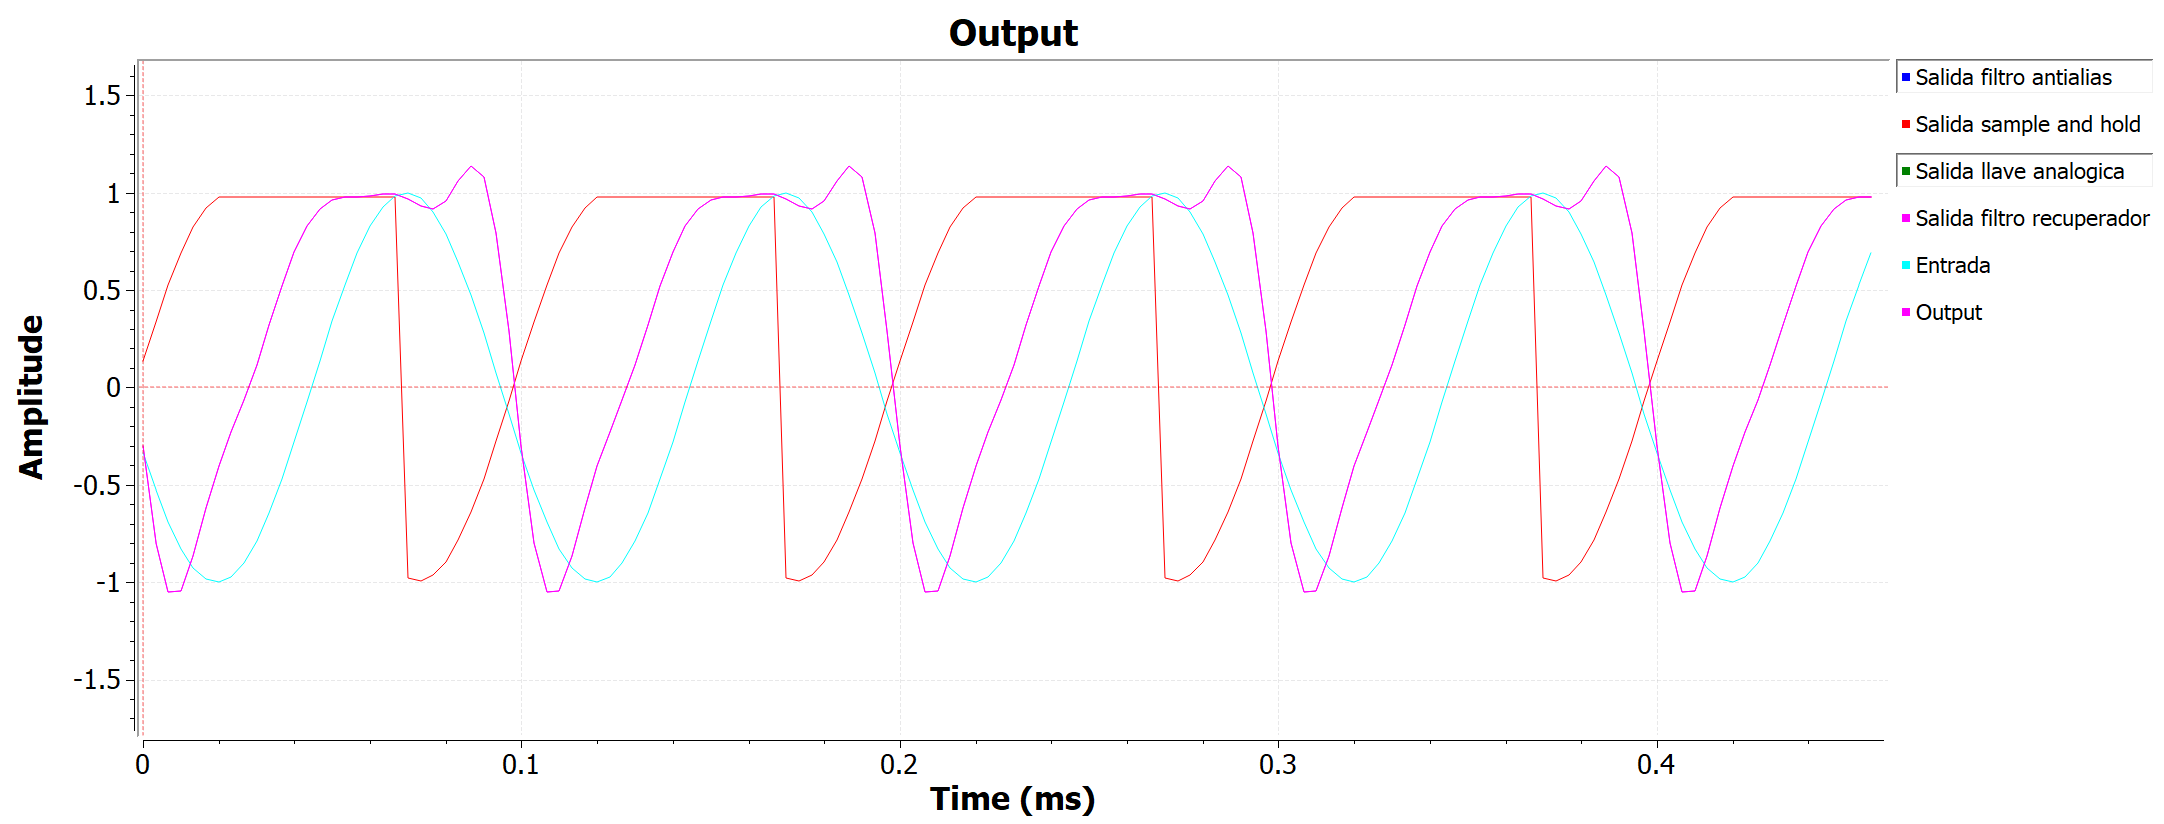
\includegraphics[scale=0.5]{Imagenes/simulacion_syh_seno_c.PNG}\caption{Simulación de la señal $X_{a}$.}
\par\end{centering}
\end{figure}

Nuevamente, al igual que en el insciso en el cual usamos la llave
analógica, la forma de la función resultante es la misma con la salvedad
que posee otro desfasaje.

\subsection{Aliasing}

Para esta úlitma medición con la llave analógica, se exitó al circuito
con las señales $X_{b}$ y $X_{c}$ variando sus frecuencias $f_{in}$
de manera tal de poder encontrar a qué frecuencia comienzan a aparecer
problemas de aliasing. Configurando la señales a una $f_{in}=2.5kHz,$observamos
que el efecto de aliasing aparece para la señal $X_{b}$ cuando $f_{s}<6kHz$
mientras que para la señal $X_{c}$aparece cuando $f_{s}<44kHz$.
Podemos ver los efectos en la siguiente imagen:

\begin{figure}[H]
\begin{centering}
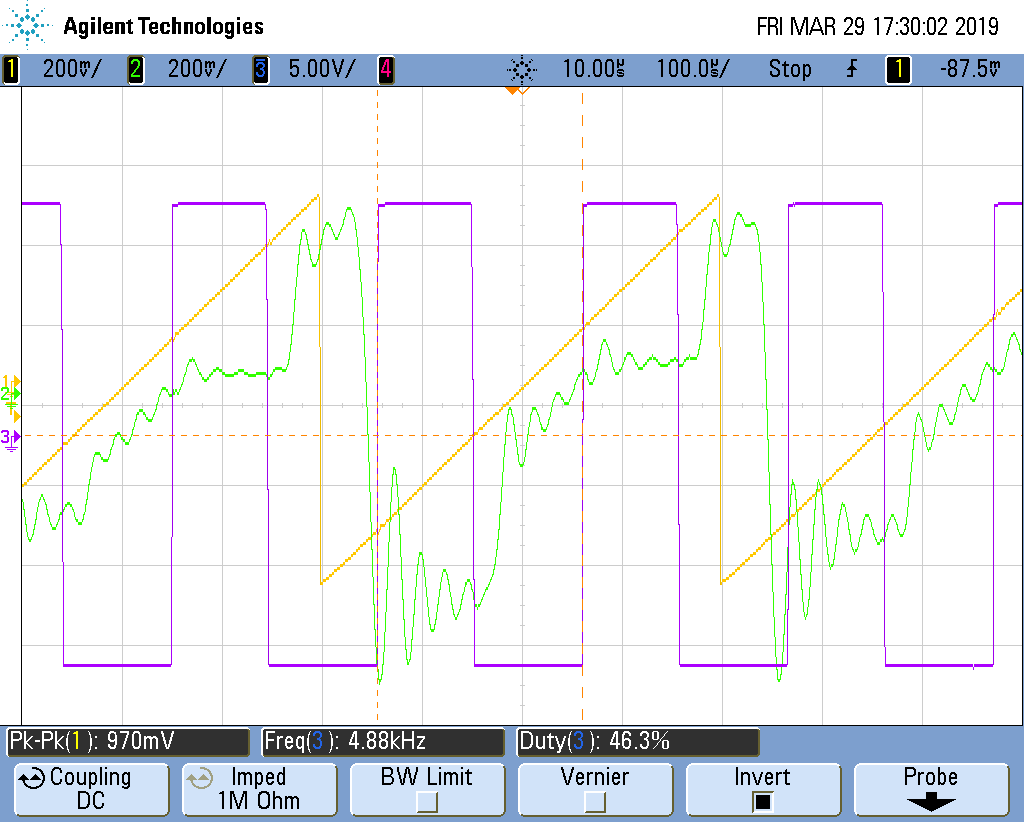
\includegraphics[scale=0.25]{Imagenes/yh_pt6d_cuad2}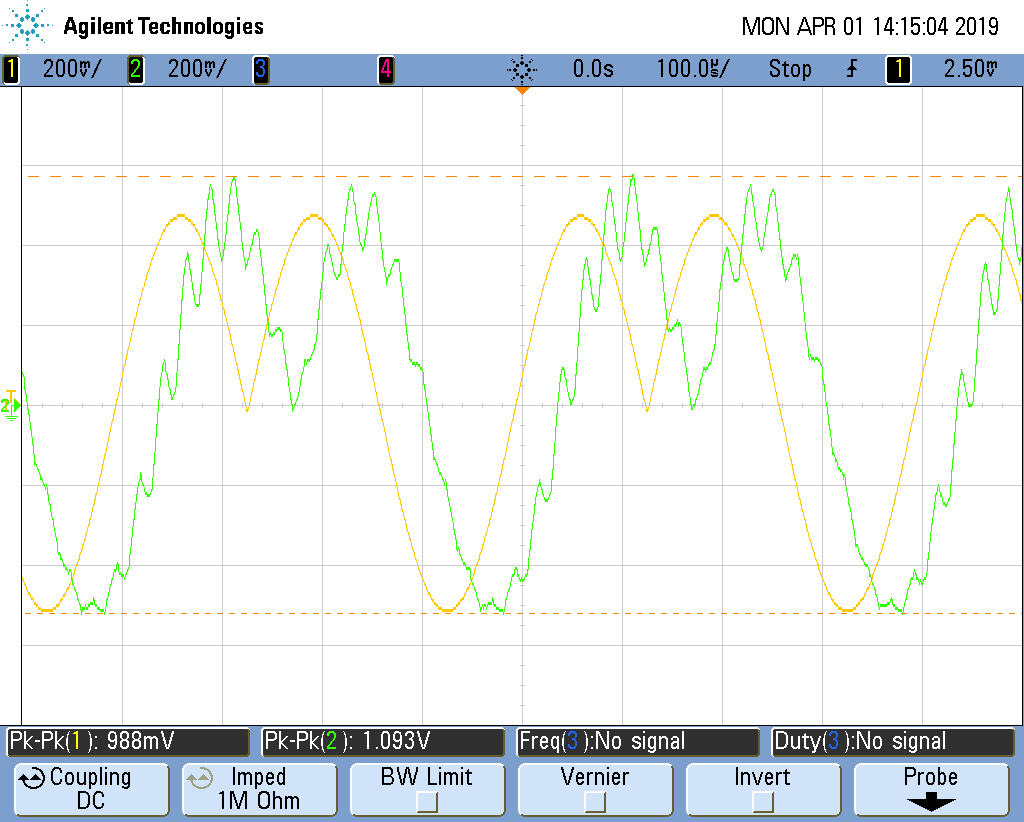
\includegraphics[scale=0.25]{Imagenes/ej_6_d_syh}
\par\end{centering}
\caption{Señal muestreada con una señal de 6kHz.}
\end{figure}

Ahora, la simulación nos entrega la siguiente gráfica:

\begin{figure}[H]

\begin{centering}
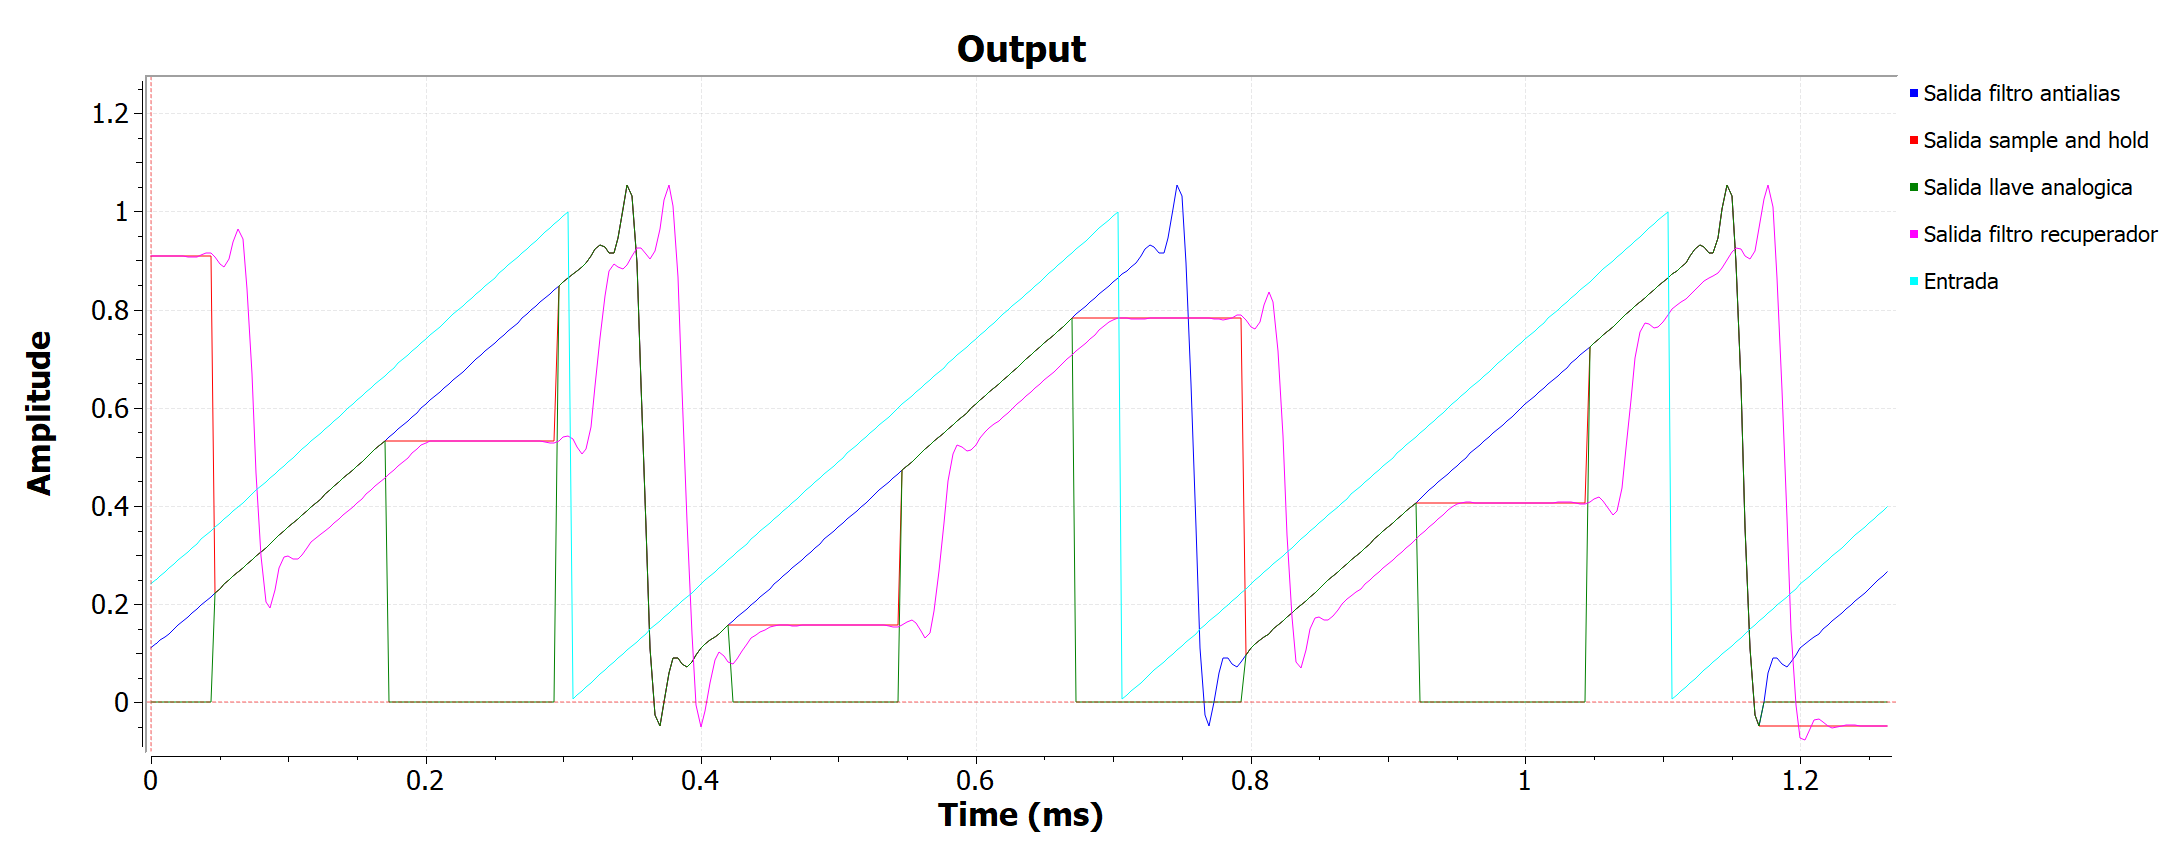
\includegraphics[scale=0.5]{Imagenes/simulacion_syh_diente_d.PNG}
\par\end{centering}
\begin{centering}
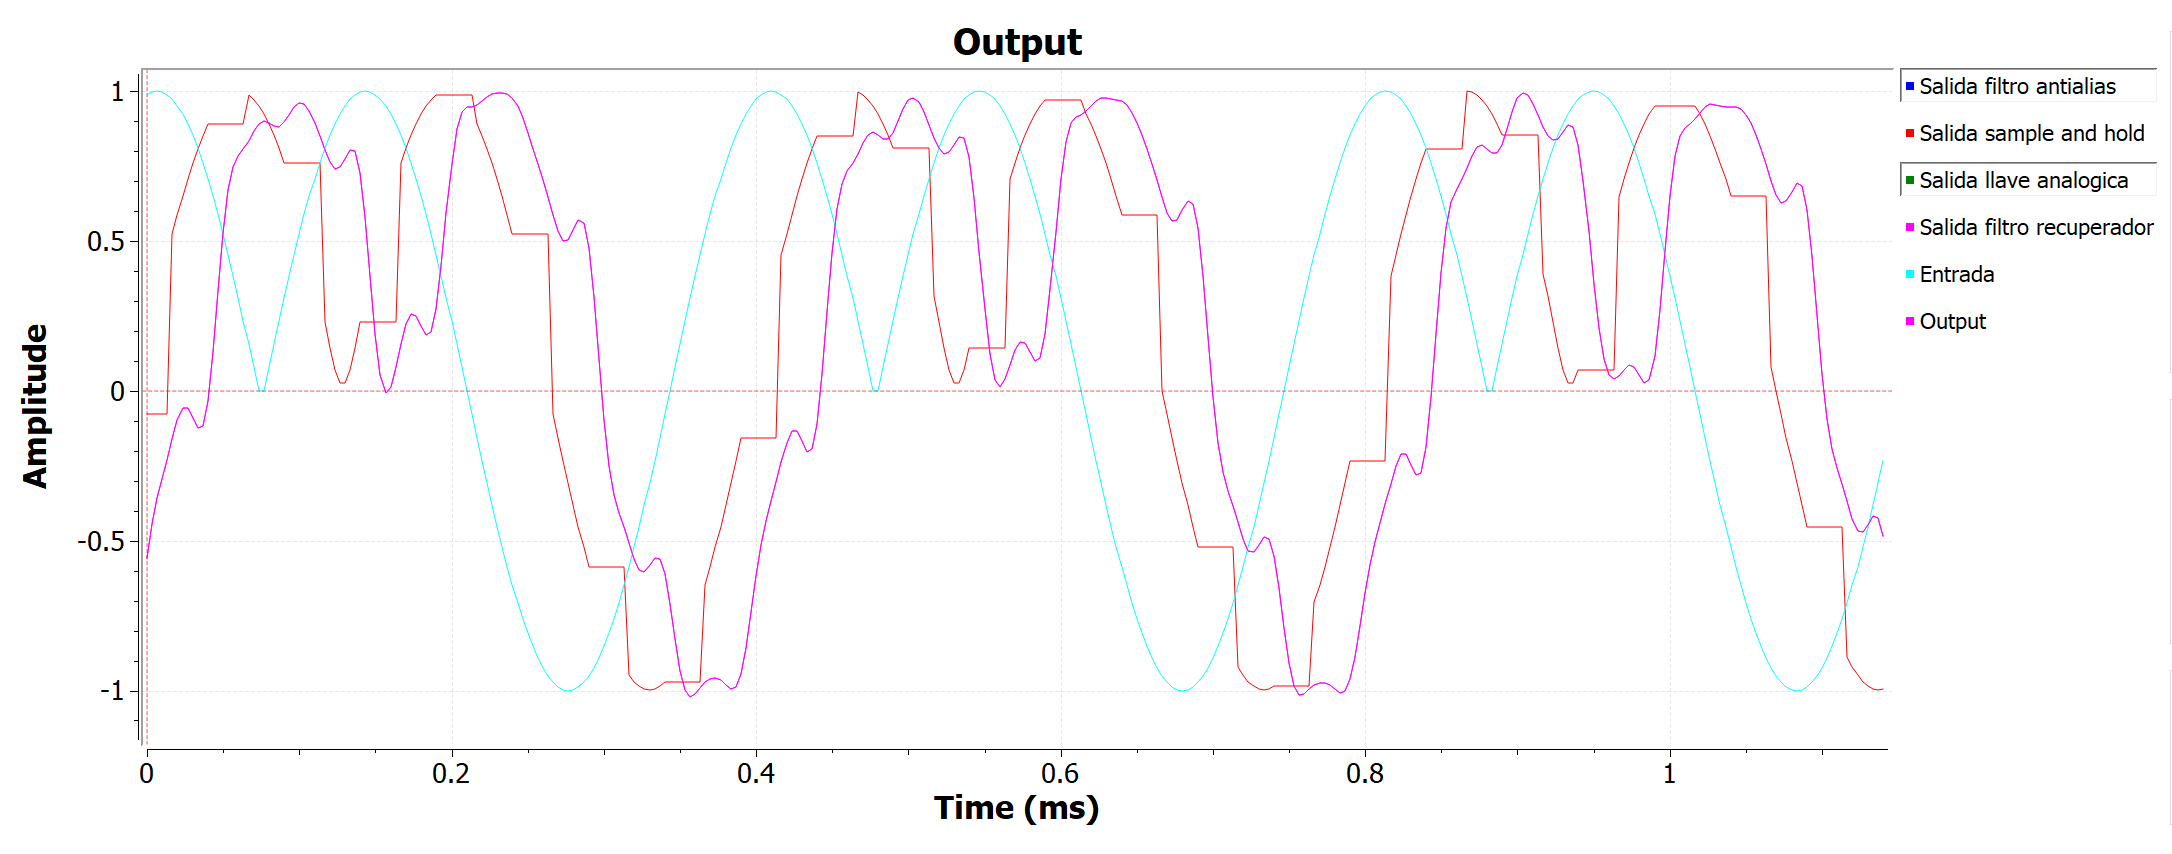
\includegraphics[scale=0.5]{Imagenes/simulacion_syh_senoraro_d.PNG}\caption{Señal simulada a iguales condiciones.}
\par\end{centering}
\end{figure}

A diferencia de lo que pasaba con la llave analógica, vemos que aquí
también la simulación posee aliasing, por lo que la figura de la señal
se ve alterada y deformada. La forma propiamente obtenida en la simulación
es similar a la obtenida en el osciloscopio.
\end{document}
